\documentclass[12pt, openany, oneside]{book}

\usepackage{listings}
\usepackage[dvipsnames]{xcolor}
\usepackage{ctex}
\usepackage{fontspec}
\usepackage{setspace}
\usepackage{tikz}
\usepackage{anyfontsize}
\usepackage{sectsty}
\usepackage{titlesec}
\usepackage{float}
\usepackage[hidelinks]{hyperref}
\usepackage[a4paper]{geometry}
\usepackage{url}
\usepackage{amssymb}
\usepackage{fontawesome5}
\usepackage[most]{tcolorbox}
\usepackage{stackengine}
\usepackage{multirow}
\usepackage[T1]{fontenc}
\usepackage{diagbox}
\usepackage{longtable}
\usepackage{newtxtt}
\usepackage{pgf-umlcd}
\usepackage{bbding}
\usepackage[edges]{forest}

\usetikzlibrary{calc,trees,positioning,arrows,fit,shapes}
\usetikzlibrary{shapes.multipart,chains}
\usetikzlibrary{shadows}

\makeatletter
\newcommand{\verbatimfont}[1]{\renewcommand{\verbatim@font}{\ttfamily#1}}
\makeatother

\tikzstyle{startend} = [rectangle, rounded corners, minimum width=3cm, minimum height=1cm, text centered, draw=black, fill=red!30]
\tikzstyle{io}        = [trapezium, trapezium left angle=70, trapezium right angle=110, minimum width=3cm, inner xsep = -15pt, minimum height=1cm, text centered, draw=black, fill=blue!30]
\tikzstyle{process}   = [rectangle, minimum width=3cm, minimum height=1cm, inner ysep=0, text centered, draw=black, fill=orange!30]
\tikzstyle{decision}  = [diamond,shape aspect=2.5, minimum width=3cm, minimum height=1cm, inner xsep=0,text centered, draw=black, fill=green!30]
\tikzstyle{arrow}     = [thick,->,>=stealth]

\def\rlwd{.5pt} \def\rlht{2.2ex} \def\rldp{.5ex}
\def\mydiv#1{~
  \rule[-\rldp]{\rlwd}{\rlht}
  \setbox0=\hbox{~#1}
  \stackunder[\dimexpr\rldp-\rlwd]{~#1}{\rule{\wd0}{\rlwd}}%
}

\definecolor{mycolor}{RGB}{0,128,128}
\newtcbox{\mybox} {
    on line,
    colback=mycolor,
    fontupper=\bfseries\color{white},
    boxrule=0pt,
    arc=5pt, 
    boxsep=0pt, 
    left=2pt, 
    right=2pt, 
    top=5pt, 
    bottom=5pt
}

\setstretch{1.5}
\setlength{\parindent}{0cm}

\geometry{a4paper,top=2.5cm,bottom=2.5cm}

\titleformat{\chapter}{\Huge\Huge\bfseries}{\chaptertitlename\ \thechapter{\ }}{0pt}{\Huge}{}
\titlespacing{\chapter}{0pt}{0pt}{12pt}

\definecolor{dkgreen}{rgb}{0,0.4,0}
\definecolor{gray}{rgb}{0.5,0.5,0.5}
\definecolor{mauve}{rgb}{0.58,0,0.82}
\definecolor{LightGray}{gray}{0.9}

\lstset{
    basicstyle=\linespread{1.3} \fontspec{Consolas},    %  the size of the fonts that are used for the code
	basewidth=0.5em,
    numbers=left,            % where to put the line-numbers
    numberstyle=\color{black},  % the style that is used for the line-numbers
    numbersep=10pt,                  % how far the line-numbers are from the code
    backgroundcolor=\color{white},
    showspaces=false,
    showstringspaces=false,
    showtabs=false,
    frame=single,                   % adds a frame around the code
    rulecolor=\color{black},        % if not set, the frame-color may be changed on line-breaks within not-black text (e.g. commens (green here))
    tabsize=4,                      % sets default tabsize to 2 spaces
    captionpos=t,                   % sets the caption-position to bottom
    breaklines=false,                % sets automatic line breaking
    breakatwhitespace=true,        % sets if automatic breaks should only happen at whitespace
    title=\lstname,                   % show the filename of files included with \lstinputlisting;
    % also try caption instead of title
    numberstyle=\color{black},		% line number color
    keywordstyle=\color{blue},          % keyword style
    commentstyle=\color{dkgreen},       % comment style
    stringstyle=\color{mauve},         % string literal style
    escapeinside={\%*}{*)},            % if you want to add LaTeX within your code
    morekeywords={*,...}               % if you want to add more keywords to the set
}

\begin{document}

\thispagestyle{empty}

\begin{tikzpicture}[overlay,remember picture]
	\fill[
		black!2]
	(current page.south west) rectangle (current page.north east);

	\shade[
		left color=Dandelion,
		right color=Dandelion!40,
		transform canvas ={rotate around ={45:($(current page.north west)+(0,-6)$)}}]
	($(current page.north west)+(0,-6)$) rectangle ++(9,1.5);

	\shade[
		left color=lightgray,
		right color=lightgray!50,
		rounded corners=0.75cm,
		transform canvas ={rotate around ={45:($(current page.north west)+(.5,-10)$)}}]
	($(current page.north west)+(0.5,-10)$) rectangle ++(15,1.5);

	\shade[
		left color=lightgray,
		rounded corners=0.3cm,
		transform canvas ={rotate around ={45:($(current page.north west)+(.5,-10)$)}}] ($(current page.north west)+(1.5,-9.55)$) rectangle ++(7,.6);

	\shade[
		left color=orange!80,
		right color=orange!60,
		rounded corners=0.4cm,
		transform canvas ={rotate around ={45:($(current page.north)+(-1.5,-3)$)}}]
	($(current page.north)+(-1.5,-3)$) rectangle ++(9,0.8);

	\shade[
		left color=red!80,
		right color=red!80,
		rounded corners=0.9cm,
		transform canvas ={rotate around ={45:($(current page.north)+(-3,-8)$)}}] ($(current page.north)+(-3,-8)$) rectangle ++(15,1.8);

	\shade[
		left color=orange,
		right color=Dandelion,
		rounded corners=0.9cm,
		transform canvas ={rotate around ={45:($(current page.north west)+(4,-15.5)$)}}]
	($(current page.north west)+(4,-15.5)$) rectangle ++(30,1.8);

	\shade[
		left color=RoyalBlue,
		right color=Emerald,
		rounded corners=0.75cm,
		transform canvas ={rotate around ={45:($(current page.north west)+(13,-10)$)}}]
	($(current page.north west)+(13,-10)$) rectangle ++(15,1.5);

	\shade[
		left color=lightgray,
		rounded corners=0.3cm,
		transform canvas ={rotate around ={45:($(current page.north west)+(18,-8)$)}}]
	($(current page.north west)+(18,-8)$) rectangle ++(15,0.6);

	\shade[
		left color=lightgray,
		rounded corners=0.4cm,
		transform canvas ={rotate around ={45:($(current page.north west)+(19,-5.65)$)}}]
	($(current page.north west)+(19,-5.65)$) rectangle ++(15,0.8);

	\shade[
		left color=OrangeRed,
		right color=red!80,
		rounded corners=0.6cm,
		transform canvas ={rotate around ={45:($(current page.north west)+(20,-9)$)}}]
	($(current page.north west)+(20,-9)$) rectangle ++(14,1.2);

	% Title
	\node[align=center] at ($(current page.center)+(0,-5)$)
	{
	{\fontsize{72}{72} \selectfont {{Java}}}\\[2cm]
	{\fontsize{20}{19.2} \selectfont \textcolor{orange}{ \bf 极夜酱}}\\[4pt]
	};
\end{tikzpicture}

\newpage

\pagestyle{plain}
\setcounter{page}{1}
\setcounter{tocdepth}{1}
\tableofcontents

\newpage

\setcounter{page}{1}

\chapter{Java简介}

\section{编程简介}

\subsection{编程简介}

程序(program)是为了让计算机执行某些操作或者解决问题而编写的一系列有序指令的集合。由于计算机只能够识别二进制数字0和1,因此需要使用特殊的编程语言来描述如何解决问题过程和方法。\\

算法(algorithm)是可完成特定任务的一系列步骤,算法的计算过程定义明确,通过一些值作为输入并产生一些值作为输出。\\

流程图(flow chart)是算法的一种图形化表示方式,使用一组预定义的符号来说明如何执行特定任务。

\begin{itemize}
	\item 圆角矩形:开始和结束
	\item 矩形:数据处理
	\item 平行四边形:输入/输出
	\item 菱形:分支判断条件
	\item 流程线:步骤
\end{itemize}

\begin{figure}
	\centering
	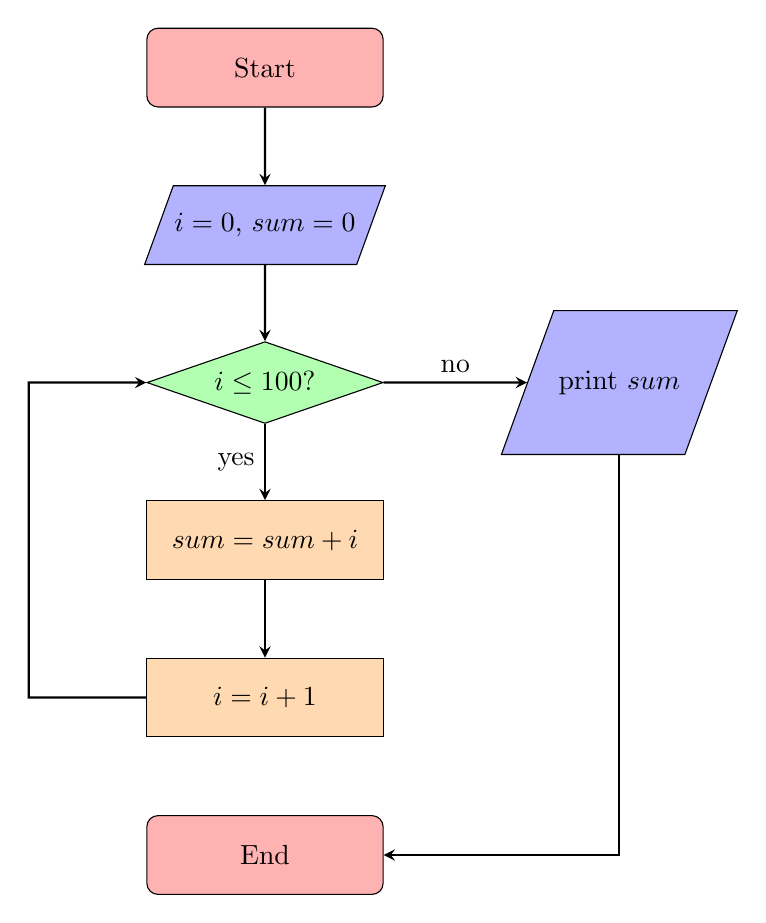
\begin{tikzpicture}[node distance=2cm]
		\node (start) [startend] {Start};
		\node (init)   [io, below of=start] {$ i = 0 $, $ sum = 0 $};
		\node (decision)  [decision, below of=init] {$ i \le 100 $?};
		\node (accumulation) [process, below of=decision] {$ sum = sum + i $};
		\node (update) [process, below of=accumulation] {$ i = i + 1 $};
		\node (output) [io, right of=decision, xshift=2.5cm] {print $ sum $};
		\node (end) [startend, below of=update] {End};

		\draw [arrow] (start) -- (init);
		\draw [arrow] (init) -- (decision);
		\draw [arrow] (decision) -- node[anchor=east] {yes } (accumulation);
		\draw [arrow] (accumulation) -- (update);
		\draw [arrow] (update) -- (-3,-8) -- (-3,-4) -- (decision);
		\draw [arrow] (decision) -- node[anchor=south] {no} (output);
		\draw [arrow] (output) |- (end);
	\end{tikzpicture}
	\caption{计算$ \sum_{i=1}^{100} i $的流程图}
\end{figure}

\vspace{0.5cm}

\subsection{编程语言(Programming Language)}

编程语言主要分为面向机器、面向过程和面向对象三类。C语言是面向过程的语言,常用于操作系统、嵌入式系统、驱动程序、图形引擎、图像处理、声音效果等。\\

Java是面向对象语言,吸收了C/C++的优点,并摒弃了难以理解的多继承、指针等概念。Java可以编写桌面应用程序、Web应用程序、分布式系统和嵌入式系统应用程序等。

\begin{figure}[H]
	\centering
	
\includegraphics[scale=0.9]{img/C1/1-1/1.png}
	\caption{常见编程语言}
\end{figure}

\newpage

\section{Hello World!}

\subsection{Hello World!}

\mybox{Hello World!}

\begin{lstlisting}[language=Java]
public class HelloWorld {
    public static void main(String[] args) {
        System.out.println("Hello World!");
    }
}
\end{lstlisting}

\begin{tcolorbox}
	\mybox{运行结果}
	\begin{verbatim}
Hello World!
	\end{verbatim}
\end{tcolorbox}

第一行语句中的public为访问修饰符,一共有三种:public、private、protected。第一行中class表示一个类,类名需要与文件名相同。\\

第二行中的main()是程序的入口。\\

第三行的语句System.out.println()的作用是在屏幕上输出“Hello World”这个字符串。【;】表示语句结束,注意不要使用中文的分号。\\

\subsection{字节码文件}

Java编译器(compiler)的作用是将Java源程序编译成中间代码字节码文件。字节码文件是一种和任何具体机器环境及操作系统环境无关的中间代码。Java程序不能直接运行在现有的操作系统,必须运行在Java虚拟机上。Java的特点是一次编写,到处运行。

\newpage

\section{Error or Warning?}

\subsection{Error / Warning}

在编写程序的过程中,错误是不可避免的,错误主要能够分为以下三种类别:

\begin{enumerate}
	\item 语法错误(syntax error):程序的语法不合符编程语言的要求,编译器会反馈报错信息。

	\item 逻辑错误(logical error):人类在编程过程中的逻辑错误,无法被编译器所检测。

	\item 运行时错误(runtime error)例如除以0、数组越界、指针越界、使用已经释放的空间、栈溢出等情况,可以被编译器发现。
\end{enumerate}

\newpage

\section{注释}

\subsection{注释(Comment)}

在编程中加入注释可以增加程序的可读性和可维护性,编译器不会对注释的部分进行编译。\\

Java中注释分为两类:

\begin{enumerate}
	\item 单行注释:将一行内【//】之后的内容视为注释。
	\item 多行注释:以【/*】开始,【*/】结束,中间的内容视为注释。
\end{enumerate}

\mybox{注释}

\begin{lstlisting}[language=Java]
/*
	这个程序在屏幕上输出Hello World
*/
public class Comment {
	// 主函数
	public static void main(String[] args) {
		System.out.println("Hello World!");		// 输出
	}
}
\end{lstlisting}

\begin{tcolorbox}
	\mybox{运行结果}
	\begin{verbatim}
Hello World!
	\end{verbatim}
\end{tcolorbox}

\newpage

\section{不同语言的Hello World}

\subsection{编程语言对比}

\mybox{C}

\begin{lstlisting}[language=C]
#include <stdio.h>

int main() {
	printf("Hello World\n");
	return 0;
}
\end{lstlisting}

\vspace{0.5cm}

\mybox{C++}

\begin{lstlisting}[language=C++]
#include <iostream>
using namespace std;

int main() {
	cout << "Hello World" << endl;
	return 0;
}
\end{lstlisting}

\vspace{0.5cm}

\mybox{Python}

\begin{lstlisting}[language=Python]
print("Hello World")
\end{lstlisting}

\newpage
\chapter{分支}

\section{逻辑运算符}

\subsection{关系运算符}

编程中经常需要使用关系运算符来比较两个数据的大小,比较的结果是一个布尔值(boolean),即True(非0)或False(0)。\\

在编程中需要注意,一个等号=表示赋值运算,而两个等号==表示比较运算。\\

\begin{table}[H]
	\centering
	\setlength{\tabcolsep}{5mm}{
		\begin{tabular}{|c|c|}
			\hline
			\textbf{数学符号} & \textbf{关系运算符} \\
			\hline
			$ < $             & <                   \\
			\hline
			$ > $             & >                   \\
			\hline
			$ \le $           & <=                  \\
			\hline
			$ \ge $           & >=                  \\
			\hline
			$ = $             & ==                  \\
			\hline
			$ \ne $           & !=                  \\
			\hline
		\end{tabular}
	}
\end{table}

\vspace{0.5cm}

\subsection{逻辑运算符}

逻辑运算符用于连接多个关系表达式,其结果也是一个布尔值。\\

\begin{enumerate}
	\item 逻辑与\&\&:当多个条件全部为True,结果为True。\\
	      \begin{table}[H]
		      \centering
		      \setlength{\tabcolsep}{5mm}{
			      \begin{tabular}{|c|c|c|}
				      \hline
				      \textbf{条件1} & \textbf{条件2} & \textbf{条件1 \&\& 条件2} \\
				      \hline
				      T              & T              & T                         \\
				      \hline
				      T              & F              & F                         \\
				      \hline
				      F              & T              & F                         \\
				      \hline
				      F              & F              & F                         \\
				      \hline
			      \end{tabular}
		      }
	      \end{table}

	\item 逻辑或||:多个条件至少有一个为True时,结果为True。\\
	      \begin{table}[H]
		      \centering
		      \setlength{\tabcolsep}{5mm}{
			      \begin{tabular}{|c|c|c|}
				      \hline
				      \textbf{条件1} & \textbf{条件2} & \textbf{条件1 || 条件2} \\
				      \hline
				      T              & T              & T                       \\
				      \hline
				      T              & F              & T                       \\
				      \hline
				      F              & T              & T                       \\
				      \hline
				      F              & F              & F                       \\
				      \hline
			      \end{tabular}
		      }
	      \end{table}

	\item 逻辑非!:条件为True时,结果为False;条件为False时,结果为True。\\
	      \begin{table}[H]
		      \centering
		      \setlength{\tabcolsep}{5mm}{
			      \begin{tabular}{|c|c|}
				      \hline
				      \textbf{条件} & \textbf{!条件} \\
				      \hline
				      T             & F              \\
				      \hline
				      F             & T              \\
				      \hline
			      \end{tabular}
		      }
	      \end{table}
\end{enumerate}

\newpage

\section{if}

\subsection{if}

if语句用于判断一个条件是否成立,如果成立则进入语句块,否则不执行。\\

\mybox{年龄}

\begin{lstlisting}[language=Java]
import java.util.Scanner;

public class Age {
	public static void main(String[] args) {
		Scanner scanner = new Scanner(System.in);

		System.out.print("Enter your age: ");
		int age = scanner.nextInt();

		if (age > 0 && age < 18) {
			System.out.println("Minor");
		}

		scanner.close();
	}
}
\end{lstlisting}

\begin{tcolorbox}
	\mybox{运行结果}
	\begin{verbatim}
Enter your age: 17
Minor
\end{verbatim}
\end{tcolorbox}

\vspace{0.5cm}

\subsection{if-else}

if-else的结构与if类似,只是在if语句块中的条件不成立时,执行else语句块中的语句。\\

\mybox{闰年}

\begin{lstlisting}[language=Java]
import java.util.Scanner;

public class Leap {
	public static void main(String[] args) {
		Scanner scanner = new Scanner(System.in);

		System.out.print("Enter a year: ");
		int year = scanner.nextInt();

		/*
			* A year is a leap year if it is
			* 1. exactly divisible by 4, and not divisible by 100;
			* 2. or is exactly divisible by 400
			*/
		if ((year % 4 == 0 && year % 100 != 0) || year % 400 == 0) {
			System.out.println("Leap year");
		} else {
			System.out.println("Common year");
		}

		scanner.close();
	}
}
\end{lstlisting}

\begin{tcolorbox}
	\mybox{运行结果}
	\begin{verbatim}
Enter a year: 2020
Leap year
\end{verbatim}
\end{tcolorbox}

\vspace{0.5cm}

\subsection{if-else if-else}

当需要对更多的条件进行判断时,可以使用if-else if-else语句。\\

\mybox{字符}

\begin{lstlisting}[language=Java]
import java.util.Scanner;

public class Character {
	public static void main(String[] args) {
		Scanner scanner = new Scanner(System.in);

		System.out.print("Enter a character: ");
		char c = scanner.next().charAt(0);

		if (c >= 'a' && c <= 'z') {
			System.out.println("Lowercase");
		} else if (c >= 'A' && c <= 'Z') {
			System.out.println("Uppercase");
		} else if (c >= '0' && c <= '9') {
			System.out.println("Digit");
		} else {
			System.out.println("Special character");
		}
		scanner.close();
	}
}	
\end{lstlisting}

\begin{tcolorbox}
	\mybox{运行结果}
	\begin{verbatim}
Enter a character: T
Uppercase
\end{verbatim}
\end{tcolorbox}

\newpage

\section{switch}

\subsection{switch}

switch结构用于根据一个整数值,选择对应的case执行。需要注意的是,当对应的case中的代码被执行完后,并不会像if语句一样跳出switch结构,而是会继续向后执行,直到遇到break。\\

\mybox{计算器}

\begin{lstlisting}[language=Java]
import java.util.Scanner;

public class Calculator {
	public static void main(String[] args) {
		Scanner scanner = new Scanner(System.in);

		System.out.print("Enter an expression: ");
		int num1 = scanner.nextInt();
		char operator = scanner.next().charAt(0);
		int num2 = scanner.nextInt();
		scanner.close();

		switch (operator) {
		case '+':
			System.out.printf(
					"%d + %d = %d\n", num1, num2, num1 + num2
			);
			break;
		case '-':
			System.out.printf(
					"%d - %d = %d\n", num1, num2, num1 - num2
			);
			break;
		case '*':
			System.out.printf(
					"%d * %d = %d\n", num1, num2, num1 * num2
			);
			break;
		case '/':
			System.out.printf(
					"%d / %d = %d\n", num1, num2, num1 / num2
			);
			break;
		default:
			System.out.println("Error! Operator is not supported");
			break;
		}
	}
}
\end{lstlisting}

\begin{tcolorbox}
	\mybox{运行结果}
	\begin{verbatim}
Enter an expression: 5 * 8
5 * 8 = 40
\end{verbatim}
\end{tcolorbox}

\newpage
\chapter{循环}

\section{自增/自减运算符}

\subsection{自增/自减运算符}

单目运算符中自增++和自减--运算符可以将变量的值加1和减1,但是++和--可以出现在变量之前或之后,即有四种情况:

\begin{enumerate}
    \item 前缀自增
    \item 前缀自减
    \item 后缀自增
    \item 后缀自减
\end{enumerate}

\begin{table}[H]
    \centering
    \setlength{\tabcolsep}{5mm}{
        \begin{tabular}{|c|l|}
            \hline
            \textbf{表达式} & \textbf{含义}        \\
            \hline
            count++         & 执行完所在语句后自增 \\
            \hline
            ++count         & 执行所在语句前自增   \\
            \hline
            count--         & 执行完所在语句后自减 \\
            \hline
            --count         & 执行所在语句前自减   \\
            \hline
        \end{tabular}
    }
    \caption{自增/自减运算符}
\end{table}

\newpage

\section{while}

\subsection{while}

在while循环中,当条件满足时重复循环体内的语句。如果条件永远为真,循环会永无止境的进行下去(死循环),因此循环体内要有改变条件的机会。\\

控制循环次数的方法就是设置循环变量:初值、判断、更新。\\

while循环的特点是先判断、再执行,所以循环体有可能会进入一次或多次,也有可能一次也不会进入。

\vspace{-0.5cm}

\begin{lstlisting}[language=Java]
while(条件) {
    // code
}
\end{lstlisting}

\vspace{0.5cm}

\mybox{计算5个人的平均身高}

\begin{lstlisting}[language=Java]
import java.util.Scanner;

public class Height {
    public static void main(String[] args) {
        Scanner scanner = new Scanner(System.in);
        double height;
        double total = 0;
        double average;
        int i = 1;
        
        while(i <= 5) {
            System.out.print("输入第" + i + "个人的身高:");
            height = scanner.nextDouble();
            total += height;
            i++;
        }
        
        average = total / 5;
        System.out.println(String.format("平均身高:%.2f", average));
        scanner.close();
    }
}
\end{lstlisting}

\begin{tcolorbox}
    \mybox{运行结果}
    \begin{verbatim}
输入第1个人的身高:160.8
输入第2个人的身高:175.2
输入第3个人的身高:171.2
输入第4个人的身高:181.3
输入第5个人的身高:164
平均身高:170.5
\end{verbatim}
\end{tcolorbox}

\newpage

\section{do-while}

\subsection{do-while}

do-while循环在进入循环的时候不做检查,而是在执行完一轮循环体的代码之后,再来检查循环的条件是否满足,如果满足则继续下一轮循环,不满足则结束循环,即至少执行一次循环。\\

do-while循环的主要特点是先执行、再判断。

\vspace{-0.5cm}

\begin{lstlisting}[language=Java]
do {
    // code
} while(条件);
\end{lstlisting}

\vspace{0.5cm}

\mybox{计算整数位数}

\begin{lstlisting}[language=Java]
import java.util.Scanner;

public class Digits {
    public static void main(String[] args) {
        Scanner scanner = new Scanner(System.in);
        int num;
        int n = 0;      // 位数
        
        System.out.print("输入整数:");
        num = scanner.nextInt();
        
        do {
            num /= 10;
            n++;
        } while(num != 0);
        
        System.out.println("位数:" + n);
        scanner.close();
    }
}
\end{lstlisting}

\begin{tcolorbox}
    \mybox{运行结果}
    \begin{verbatim}
输入整数:123
位数:3
\end{verbatim}
\end{tcolorbox}

\vspace{0.5cm}

\subsection{while与do-while区别}

while循环与do-while循环有以下区别:

\begin{enumerate}
    \item 执行顺序不同。

    \item 初始情况不满足循环条件时,while循环一次都不会执行,do-while循环不管任何情况都至少执行一次。

    \item do-while循环的while语句后有【;】。
\end{enumerate}

\begin{figure}[H]
    \centering
    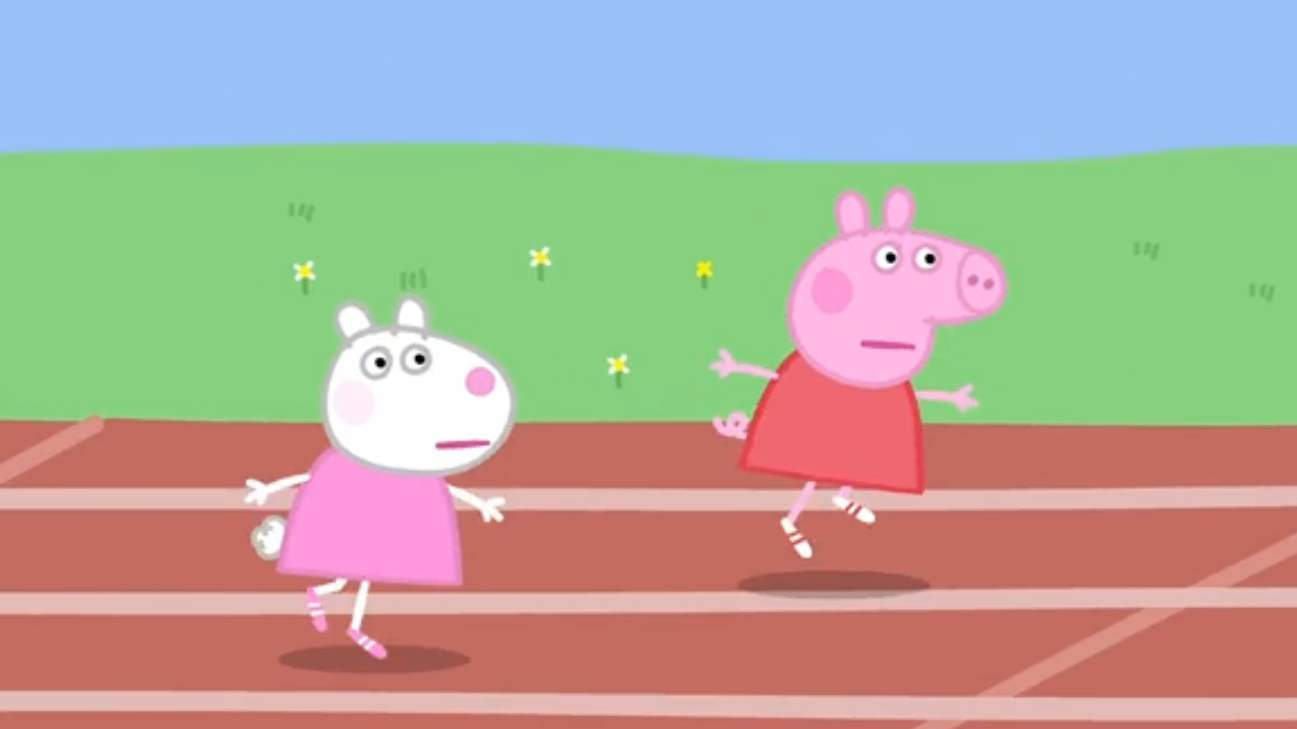
\includegraphics[scale=0.15]{img/Chapter4/4-3/1.png}
\end{figure}

\mybox{猜数字}

\begin{lstlisting}[language=Java]
import java.util.Scanner;

public class GuessNumber {
    public static void main(String[] args) {
        Scanner scanner = new Scanner(System.in);
        int answer = (int)(Math.random() * 100) + 1;    // [1, 100]
        int guess;
        int cnt = 0;        // 猜测次数
        
        do {
            System.out.print("猜一个1-100之间的数:");
            guess = scanner.nextInt();
            cnt++;
            if(guess < answer) {
                System.out.println("猜小啦!");
            } else if(guess > answer) {
                System.out.println("猜大啦!");
            }
        } while(guess != answer);
        
        System.out.println("猜对啦!一共猜了" + cnt + "次!");
        scanner.close();
    }
}
\end{lstlisting}

\begin{tcolorbox}
    \mybox{运行结果}
    \begin{verbatim}
猜一个1-100之间的数字:50
猜大了!
猜一个1-100之间的数字:25
猜小了!
猜一个1-100之间的数字:37
猜小了!
猜一个1-100之间的数字:43
猜小了!
猜一个1-100之间的数字:46
猜小了!
猜一个1-100之间的数字:48
猜小了!
猜一个1-100之间的数字:49
猜对了!你一共用了7次猜对!
\end{verbatim}
\end{tcolorbox}

\newpage

\section{for}

\subsection{for}

for循环有三个表达式,中间用【;】分隔,【;】不可省略。

\vspace{-0.5cm}

\begin{lstlisting}[language=Java]
for(表达式1; 表达式2; 表达式3) {
    //code
}
\end{lstlisting}

\begin{itemize}
    \item 表达式1通常是为循环变量赋初值,可省略。
    \item 表达式2是循环条件,判断是否继续执行循环,可省略。
    \item 表达式3为更新循环变量的值,可省略。
\end{itemize}

\vspace{0.5cm}

\mybox{计算1-100的累加和}

\begin{lstlisting}[language=Java]
public class Sum {
    public static void main(String[] args) {
        int sum = 0;
        for(int i = 1; i <= 100; i++) {
            sum += i;
        }
        System.out.println(sum);
    }
}
\end{lstlisting}

\begin{tcolorbox}
    \mybox{运行结果}
    \begin{verbatim}
5050
\end{verbatim}
\end{tcolorbox}

\vspace{0.5cm}

\mybox{计算$ 1 + {1 \over 2} + {1 \over 3} + ... + {1 \over n} $}

\begin{lstlisting}[language=Java]
import java.util.Scanner;

public class InverseSum {
    public static void main(String[] args) {
        Scanner scanner = new Scanner(System.in);
        int n;
        double sum = 0.0;
        
        System.out.print("输入n:");
        n = scanner.nextInt();
        
        for(int i = 1; i <= n; i++) {
            sum += 1.0 / i;
        }
        
        System.out.println(sum);
        scanner.close();
    }
}
\end{lstlisting}

\begin{tcolorbox}
    \mybox{运行结果}
    \begin{verbatim}
输入n:10
2.928968
\end{verbatim}
\end{tcolorbox}

\vspace{0.5cm}

\mybox{斐波那契数列}

\begin{figure}[H]
    \centering
    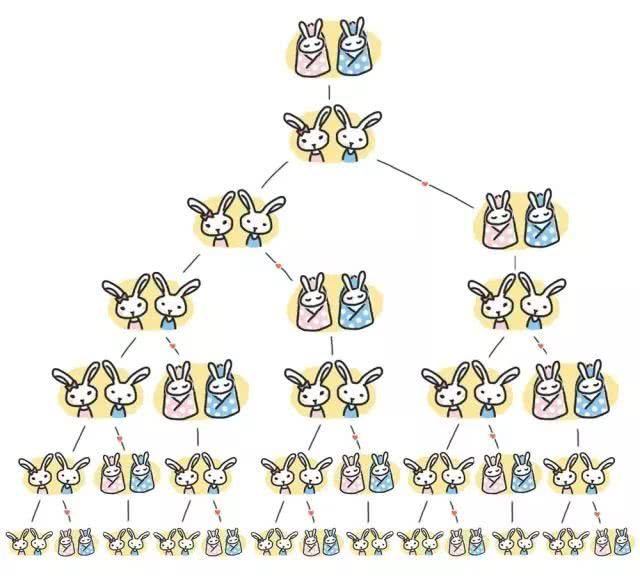
\includegraphics[scale=0.45]{img/Chapter4/4-4/1.png}
\end{figure}

\begin{lstlisting}[language=Java]
import java.util.Scanner;

public class Fibonacci {
    public static void main(String[] args) {
        Scanner scanner = new Scanner(System.in);
        int n;
        int num1, num2, val;
        
        System.out.print("输入斐波那契数列长度:");
        n = scanner.nextInt();
        
        if(n == 1) {
            System.out.println("1");
        } else if(n == 2) {
            System.out.println("1, 1");
        } else {
            num1 = 1;
            num2 = 1;
            System.out.print("1, 1");
            for(int i = 3; i <= n; i++) {
                val = num1 + num2;
                System.out.print(", " + val);
                num1 = num2;
                num2 = val;
            }
            System.out.println();
        }
        scanner.close();
    }
}
\end{lstlisting}

\begin{tcolorbox}
    \mybox{运行结果}
    \begin{verbatim}
输入斐波那契数列长度:10
1, 1, 2, 3, 5, 8, 13, 21, 34, 55
\end{verbatim}
\end{tcolorbox}

\vspace{0.5cm}

\subsection{嵌套循环}

循环也可以进行嵌套使用。\\

\mybox{九九乘法表}\\

\begin{table}[H]
    \centering
    \setlength{\tabcolsep}{1.5mm}{
        \begin{tabular}{|c|c|c|c|c|c|c|c|c|}
            \hline
            1*1=1 & 1*2=2  & 1*3=3  & 1*4=4  & 1*5=5  & 1*6=6  & 1*7=7  & 1*8=8  & 1*9=9  \\
            \hline
            2*1=2 & 2*2=4  & 2*3=6  & 2*4=8  & 2*5=10 & 2*6=12 & 2*7=14 & 2*8=16 & 2*9=18 \\
            \hline
            3*1=3 & 3*2=6  & 3*3=9  & 3*4=12 & 3*5=15 & 3*6=18 & 3*7=21 & 3*8=24 & 3*9=27 \\
            \hline
            4*1=4 & 4*2=8  & 4*3=12 & 4*4=16 & 4*5=20 & 4*6=24 & 4*7=28 & 4*8=32 & 4*9=36 \\
            \hline
            5*1=5 & 5*2=10 & 5*3=15 & 5*4=20 & 5*5=25 & 5*6=30 & 5*7=35 & 5*8=40 & 5*9=45 \\
            \hline
            6*1=6 & 6*2=12 & 6*3=18 & 6*4=24 & 6*5=30 & 6*6=36 & 6*7=42 & 6*8=48 & 6*9=54 \\
            \hline
            7*1=7 & 7*2=14 & 7*3=21 & 7*4=28 & 7*5=35 & 7*6=42 & 7*7=49 & 7*8=56 & 7*9=63 \\
            \hline
            8*1=8 & 8*2=16 & 8*3=24 & 8*4=32 & 8*5=40 & 8*6=48 & 8*7=56 & 8*8=64 & 8*9=72 \\
            \hline
            9*1=9 & 9*2=18 & 9*3=27 & 9*4=36 & 9*5=45 & 9*6=54 & 9*7=63 & 9*8=72 & 9*9=81 \\
            \hline
        \end{tabular}
    }
    \caption{九九乘法表}
\end{table}

\begin{lstlisting}[language=Java]
public class MultiplicationTable {
    public static void main(String[] args) {
        for(int i = 1; i <= 9; i++) {
            for(int j = 1; j <= 9; j++) {
                System.out.print(
                    String.format("%d*%d=%d\t", i, j, i*j)
                );
            }
            System.out.println();
        }
    }
}
\end{lstlisting}

\vspace{0.5cm}

\mybox{输出图案}

\begin{lstlisting}
*
**
***
****
*****
\end{lstlisting}

\begin{lstlisting}[language=Java]
public class Stars {
    public static void main(String[] args) {
        for(int i = 1; i <= 5; i++) {
            for(int j = 1; j <= i; j++) {
                System.out.print("*");
            }
            System.out.println();
        }
    }
}
\end{lstlisting}

\newpage

\section{break or continue?}

\subsection{循环控制}

循环控制语句的作用是控制当前的循环结构是否继续向下执行,如果不进行控制,那么会根据既定的结构重复执行。如果有一些特殊的情况导致循环的执行中断,就称为循环的控制语句。循环控制语句的关键字有break和continue。\\

break的作用是跳出当前循环,执行当前循环之后的语句。break只能跳出一层循环,如果是嵌套循环,那么需要按照嵌套的层次,逐步使用break来跳出。break语句只能在循环体内和switch语句内使用。\\

continue的作用是跳过本轮循环,开始下一轮循环的条件判断。continue终止当前轮的循环过程,但它并不跳出循环。\\

\mybox{break}

\begin{lstlisting}[language=Java]
public class Break {
    public static void main(String[] args) {
        for(int i = 1; i <= 10; i++) {
            if(i == 5) {
                break;
            }
            System.out.print(i + " ");
        }
    }
}
\end{lstlisting}

\begin{tcolorbox}
    \mybox{运行结果}
    \begin{verbatim}
1 2 3 4
\end{verbatim}
\end{tcolorbox}

\vspace{0.5cm}

\mybox{continue}

\begin{lstlisting}[language=Java]
public class Continue {
    public static void main(String[] args) {
        for(int i = 1; i <= 10; i++) {
            if(i == 5) {
                continue;
            }
            System.out.print(i + " ");
        }
    }
}
\end{lstlisting}

\begin{tcolorbox}
    \mybox{运行结果}
    \begin{verbatim}
1 2 3 4 6 7 8 9 10
\end{verbatim}
\end{tcolorbox}

\newpage
\chapter{数组}

\section{一维数组}

\subsection{数组(Array)}

一个变量只能存储一个内容,如果需要存储更多数据,就需要使用数组解决问题。一个数组变量可以存放多个数据,数组是一个值的集合,它们共享同一个名字,数组中的每个变量都能被其下标所访问。

\vspace{-0.5cm}

\begin{lstlisting}[language=Java]
int[] number = new int[10];
float[] grade = new float[50];
\end{lstlisting}

\begin{figure}[H]
	\centering
	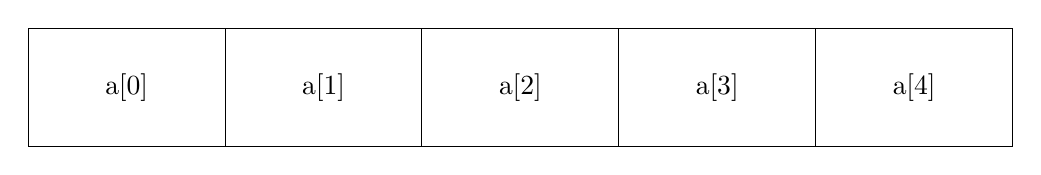
\begin{tikzpicture}[scale=0.5]
		\draw[-] (0,0) -- (5,0) -- (10,0) -- (15,0) -- (20,0) -- (25,0) -- (25,3) -- (20,3) -- (15,3) -- (10,3) -- (5,3) -- (0,3) -- (0,0);
		\draw[-] (5,0) -- (5,3);
		\draw[-] (10,0) -- (10,3);
		\draw[-] (15,0) -- (15,3);
		\draw[-] (20,0) -- (20,3);

		\draw (2.5,1.5) node {a[0]};
		\draw (7.5,1.5) node {a[1]};
		\draw (12.5,1.5) node {a[2]};
		\draw (17.5,1.5) node {a[3]};
		\draw (22.5,1.5) node {a[4]};
	\end{tikzpicture}
\end{figure}

\begin{itemize}
	\item 元素:数组中的每个变量
	\item 大小:数组的容量
	\item 下标 / 索引(index):元素的位置,下标从0开始,必须为非负整数
\end{itemize}

\vspace{0.5cm}

\subsection{数组初始化}

一维数组可以在声明时进行初始化:

\vspace{-0.5cm}

\begin{lstlisting}[language=Java]
int[] arr = {3, 6, 8, 2, 4, 0, 9, 7, 1, 5};
int[] arr = new int[] {3, 6, 8, 2, 4, 0, 9, 7, 1, 5};
\end{lstlisting}

很多时候在使用数组之前需要将数组的内容全部清空,这可以利用循环来实现。\\

\mybox{一维数组初始化}

\begin{lstlisting}[language=Java]
public class InitArr {
    public static void main(String[] args) {
        int[] arr = new int[100];
        for(int i = 0; i < arr.length; i++) {
            arr[i] = 0;
        }
    }
}
\end{lstlisting}

\vspace{0.5cm}

\mybox{数组最大值和最小值}

\begin{lstlisting}[language=Java]
public class MaxMin {
    public static void main(String[] args) {
        int[] num = {7, 6, 2, 9, 3, 1, 4, 0, 5, 8};
        int max = num[0];
        int min = num[0];

        for(int i = 1; i < num.length; i++) {
            if(num[i] > max) {
                max = num[i];
            } else if(num[i] < min) {
                min = num[i];
            }
        }

        System.out.println("max = " + max);
        System.out.println("min = " + min);
    }
}
\end{lstlisting}

\begin{tcolorbox}
	\mybox{运行结果}
	\begin{verbatim}
max = 9
min = 0
	\end{verbatim}
\end{tcolorbox}

\vspace{0.5cm}

\subsection{for-each}

for-each环是for循环的特殊简化版。

\vspace{-0.5cm}

\begin{lstlisting}[language=Java]
for(dataType var : set) {
    // code
}
\end{lstlisting}

\vspace{0.5cm}

\mybox{遍历数组}

\begin{lstlisting}[language=Java]
public class ForEach {
    public static void main(String[] args) {
        int[] arr = {7, 6, 2, 9, 3, 1, 4, 0, 5, 8};
        for(int elem : arr) {
            System.out.print(elem + " ");
        }
    }
}
\end{lstlisting}

\begin{tcolorbox}
	\mybox{运行结果}
	\begin{verbatim}
7 6 2 9 3 1 4 0 5 8
	\end{verbatim}
\end{tcolorbox}

\newpage

\section{二维数组}

\subsection{二维数组(2D Array)}

二维数组包括行和列两个维度,可以看成是由多个一维数组组成。

\begin{table}[H]
	\centering
	\setlength{\tabcolsep}{5mm}{
		\begin{tabular}{|c|c|c|c|}
			\hline
			a[0][0] & a[0][1] & a[0][2] & a[0][3] \\
			\hline
			a[1][0] & a[1][1] & a[1][2] & a[1][3] \\
			\hline
			a[2][0] & a[2][1] & a[2][2] & a[2][3] \\
			\hline
		\end{tabular}
	}
\end{table}

二维数组可以在声明时进行初始化:

\vspace{-0.5cm}

\begin{lstlisting}[language=Java]
int[][] arr = new int[2][3];
int[][] arr = {{1, 2, 3}, {4, 5, 6}};
\end{lstlisting}

\vspace{0.5cm}

\mybox{初始化二维数组}

\begin{lstlisting}[language=Java]
public class Init2dArr {
    public static void main(String[] args) {
        int[][] arr = new int[3][4];
        for(int i = 0; i < arr.length; i++) {
            for(int j = 0; j < arr[i].length; j++) {
                arr[i][j] = 0;
            }
        }
    }
}
\end{lstlisting}

\vspace{0.5cm}

\mybox{矩阵运算}

\vspace{0.5cm}

矩阵的加法/减法是指两个矩阵把其相对应元素进行加减的运算。\\

矩阵加法:两个$ m \times n $矩阵A和B的和,标记为$ A + B $,结果为一个$ m \times n $的矩阵,其内的各元素为其相对应元素相加后的值。\\

矩阵减法:两个$ m \times n $矩阵A和B的差,标记为$ A - B $,结果为一个$ m \times n $的矩阵,其内的各元素为其相对应元素相减后的值。

\begin{align}\nonumber
	\left[\begin{matrix}
			1 & 3 \\
			1 & 0 \\
			1 & 2 \\
		\end{matrix} \right]
	+
	\left[\begin{matrix}
			0 & 0 \\
			7 & 5 \\
			2 & 1 \\
		\end{matrix} \right]
	=
	\left[\begin{matrix}
			1+0 & 3+0 \\
			1+7 & 0+5 \\
			1+2 & 2+1 \\
		\end{matrix} \right]
	=
	\left[\begin{matrix}
			1 & 3 \\
			8 & 5 \\
			3 & 3 \\
		\end{matrix} \right]
\end{align}

\begin{align}\nonumber
	\left[\begin{matrix}
			1 & 3 \\
			1 & 0 \\
			1 & 2 \\
		\end{matrix} \right]
	-
	\left[\begin{matrix}
			0 & 0 \\
			7 & 5 \\
			2 & 1 \\
		\end{matrix} \right]
	=
	\left[\begin{matrix}
			1-0 & 3-0 \\
			1-7 & 0-5 \\
			1-2 & 2-1 \\
		\end{matrix} \right]
	=
	\left[\begin{matrix}
			1  & 3  \\
			-6 & -5 \\
			-1 & 1  \\
		\end{matrix} \right]
\end{align}

\begin{lstlisting}[language=Java]
public class Matrix {
    public static void main(String[] args) {
        int[][] A = {
            {1, 3},
            {1, 0},
            {1, 2}
        };
        int[][] B = {
            {0, 0},
            {7, 5},
            {2, 1}
        };
        int[][] C = new int[3][2];

        System.out.println("矩阵加法");
        for(int i = 0; i < 3; i++) {
            for(int j = 0; j < 2; j++) {
                C[i][j] = A[i][j] + B[i][j];
                System.out.print(String.format("%3d", C[i][j]));
            }
            System.out.println();
        }

        System.out.println("矩阵减法");
        for(int i = 0; i < 3; i++) {
            for(int j = 0; j < 2; j++) {
                C[i][j] = A[i][j] - B[i][j];
                System.out.print(String.format("%3d", C[i][j]));
            }
            System.out.println();
        }
    }
}
\end{lstlisting}

\begin{tcolorbox}
	\mybox{运行结果}
	\begin{verbatim}
矩阵加法
1  3
8  5
3  3
矩阵减法
1  3
-6 -5
-1  1
	\end{verbatim}
\end{tcolorbox}

\newpage

\section{字符}

\subsection{字符(Character)}

单个的字符是一种特殊的类型,是用单引号表示字符字面量。每一个字符都有其对应的码值。\\

ASCII全称American Standard Code for Information Interchange(美国信息交换标准代码),一共定义了128个字符。

\begin{longtable}{|c|c|c|c|c|c|c|c|}
	\hline
	\textbf{ASCII} & \textbf{字符} & \textbf{ASCII} & \textbf{字符} & \textbf{ASCII} & \textbf{字符}          & \textbf{ASCII} & \textbf{字符}          \\
	\hline
	0              & NUT           & 32             & (space)       & 64             & @                      & 96             & \lstinline|`| \\
	\hline
	1              & SOH           & 33             & !             & 65             & A                      & 97             & a                      \\
	\hline
	2              & STX           & 34             & \text{"}      & 66             & B                      & 98             & b                      \\
	\hline
	3              & ETX           & 35             & \#            & 67             & C                      & 99             & c                      \\
	\hline
	4              & EOT           & 36             & \$            & 68             & D                      & 100            & d                      \\
	\hline
	5              & ENQ           & 37             & \%            & 69             & E                      & 101            & e                      \\
	\hline
	6              & ACK           & 38             & \&            & 70             & F                      & 102            & f                      \\
	\hline
	7              & BEL           & 39             & \text{'}      & 71             & G                      & 103            & g                      \\
	\hline
	8              & BS            & 40             & (             & 72             & H                      & 104            & h                      \\
	\hline
	9              & HT            & 41             & )             & 73             & I                      & 105            & i                      \\
	\hline
	10             & LF            & 42             & *             & 74             & J                      & 106            & j                      \\
	\hline
	11             & VT            & 43             & +             & 75             & K                      & 107            & k                      \\
	\hline
	12             & FF            & 44             & ,             & 76             & L                      & 108            & l                      \\
	\hline
	13             & CR            & 45             & -             & 77             & M                      & 109            & m                      \\
	\hline
	14             & SO            & 46             & .             & 78             & N                      & 110            & n                      \\
	\hline
	15             & SI            & 47             & /             & 79             & O                      & 111            & o                      \\
	\hline
	16             & DLE           & 48             & 0             & 80             & P                      & 112            & p                      \\
	\hline
	17             & DC1           & 49             & 1             & 81             & Q                      & 113            & q                      \\
	\hline
	18             & DC2           & 50             & 2             & 82             & R                      & 114            & r                      \\
	\hline
	19             & DC3           & 51             & 3             & 83             & S                      & 115            & s                      \\
	\hline
	20             & DC4           & 52             & 4             & 84             & T                      & 116            & t                      \\
	\hline
	21             & NAK           & 53             & 5             & 85             & U                      & 117            & u                      \\
	\hline
	22             & SYN           & 54             & 6             & 86             & V                      & 118            & v                      \\
	\hline
	23             & TB            & 55             & 7             & 87             & W                      & 119            & w                      \\
	\hline
	24             & CAN           & 56             & 8             & 88             & X                      & 120            & x                      \\
	\hline
	25             & EM            & 57             & 9             & 89             & Y                      & 121            & y                      \\
	\hline
	26             & SUB           & 58             & :             & 90             & Z                      & 122            & z                      \\
	\hline
	27             & ESC           & 59             & ;             & 91             & [                      & 123            & \{                     \\
			\hline
	28             & FS            & 60             & <             & 92             & /                      & 124            & |                      \\
			\hline
	29             & GS            & 61             & =             & 93             & ]                      & 125            & \}                     \\
	\hline
	30             & RS            & 62             & >             & 94             & \lstinline|^| & 126            & \lstinline|~| \\
	\hline
	31             & US            & 63             & ?             & 95             & \_                     & 127            & DEL                    \\
	\hline
	\caption{ASCII码表}
\end{longtable}

\mybox{ASCII码}

\begin{lstlisting}[language=Java]
public class ASCII {
	public static void main(String[] args) {
		for(int i = 0; i < 128; i++) {
			System.out.println(String.format("%c = %d", i, i));
		}
	}
}
\end{lstlisting}

\newpage

\section{字符串}

\subsection{字符串(String)}

字符串是用双引号所表示的0个或多个字符的组合。字符串变量使用String表示,String是一个类,String的变量是对象的管理者而非所有者。

\begin{figure}[H]
	\centering
	\begin{tikzpicture}
		\draw[-] (-5,0) -- (-1,0);
		\draw[-] (1,0) -- (5,0);
		\draw (0,0) node {b = a};

		\draw (-4,-2.5) rectangle (-2,-1.5);
		\draw (2,-2.5) rectangle (4,-1.5);
		\draw (-3,-1) node {int a;};
		\draw (3,-1) node {int b;};
		\draw (-3,-2) node {32};
		\draw (3,-2) node {32};

		\draw (-4,-5.5) rectangle (-2,-4.5);
		\draw (2,-5.5) rectangle (4,-4.5);
		\draw (-3,-4) node {String a;};
		\draw (3,-4) node {String b;};

		\draw (-1,-7) rectangle (1,-6);
		\draw[->] (-2,-5) -- (-1,-6.5);
		\draw[->] (2,-5) -- (1,-6.5);
	\end{tikzpicture}
	\caption{字符串引用}
\end{figure}

通过调用Scanner类中的nextLine()可以获取用户输入的字符串。\\

\mybox{创建字符串对象}

\begin{lstlisting}[language=Java]
import java.util.Scanner;

public class StringObj {
	public static void main(String[] args) {
		Scanner scanner = new Scanner(System.in);
		System.out.print("输入字符串:");
		String str = scanner.nextLine();
		System.out.println(str);
		scanner.close();
	}
}
\end{lstlisting}

\begin{tcolorbox}
	\mybox{运行结果}
	\begin{verbatim}
输入字符串:Hello World!
Hello World!
	\end{verbatim}
\end{tcolorbox}

\vspace{0.5cm}

\subsection{字符串比较}

字符串的比较分为两种:

\begin{enumerate}
	\item 【==】运算符用于比较是否是同一个对象。
	\item equals()用于比较字符串的内容是否相同。
\end{enumerate}

\mybox{字符串比较}

\begin{lstlisting}[language=Java]
public class StringEqual {
	public static void main(String[] args) {
		String s1 = new String("hello");
		String s2 = new String("hello");

		if(s1 == s2) {
			System.out.println("s1和s2是同一个对象");
		}

		if(s1.equals(s2)) {
			System.out.println("s1与s2内容相同");
		}

		if(s1.equalsIgnoreCase(s2)) {
			System.out.println("s1与s2忽略大小写内容相同");
		}
	}
}
\end{lstlisting}

\begin{tcolorbox}
	\mybox{运行结果}
	\begin{verbatim}
s1与s2内容相同
s1与s2忽略大小写内容相同
	\end{verbatim}
\end{tcolorbox}

\vspace{0.5cm}

\subsection{字符串操作}

字符串是对象,它包含了一系列的常用操作,对它的所有操作都是通过【.】运算符进行的。

\subsubsection{length():计算字符串长度}

\vspace{0.5cm}

\mybox{计算字符串长度}

\begin{lstlisting}[language=Java]
public class StringLength {
	public static void main(String[] args) {
		String str = "Hello World!";
		System.out.println(str.length());
	}
}
\end{lstlisting}

\begin{tcolorbox}
	\mybox{运行结果}
	\begin{verbatim}
12
	\end{verbatim}
\end{tcolorbox}

\subsubsection{charAt():访问字符串中的字符}

字符串中的每一个下标位置都是一个单个的字符,下标的范围从0到length() - 1。

\vspace{0.5cm}

\mybox{访问字符串中的字符}

\begin{lstlisting}[language=Java]
public class CharAt {
	public static void main(String[] args) {
		String str = "Hello World!";
		System.out.println(str.charAt(4));
	}
}
\end{lstlisting}

\begin{tcolorbox}
	\mybox{运行结果}
	\begin{verbatim}
o
	\end{verbatim}
\end{tcolorbox}

\vspace{0.5cm}

\mybox{计算字符串中某个字符出现的次数}

\begin{lstlisting}[language=Java]
import java.util.Scanner;

public class CountOccurence {
	public static void main(String[] args) {
		Scanner scanner = new Scanner(System.in);
		int cnt = 0;		// 出现次数

		System.out.print("输入字符串:");
		String str = scanner.nextLine();
		System.out.print("输入待统计字符:");
		char c = scanner.nextLine().charAt(0);

		int n = str.length();
		for(int i = 0; i < n; i++) {
			if(str.charAt(i) == c) {
				cnt++;
			}
		}

		System.out.println(c + "在" + str + "中出现了" + cnt + "次");
		scanner.close();
	}
}
\end{lstlisting}

\begin{tcolorbox}
	\mybox{运行结果}
	\begin{verbatim}
输入字符串:Hello World
输入待统计字符:l
l在Hello World中出现了3次
	\end{verbatim}
\end{tcolorbox}

\subsubsection{substring():获取子串}

\begin{itemize}
	\item substring(n):获取第n个位置到末尾的全部内容。
	\item substring(begin, end):获取从begin到end位置之前的内容。
\end{itemize}

\mybox{获取子串}

\begin{lstlisting}[language=Java]
public class Substring {
	public static void main(String[] args) {
		String str = "Hello World!";
		System.out.println(str.substring(6));
		System.out.println(str.substring(3, 10));
	}
}
\end{lstlisting}

\begin{tcolorbox}
	\mybox{运行结果}
	\begin{verbatim}
World!
lo Worl
	\end{verbatim}
\end{tcolorbox}

\subsubsection{indexOf():查找}

\begin{itemize}
	\item indexOf(c):获取字符c所在的位置,返回-1表示不存在。
	\item indexOf(c, n):从第n个位置开始查找字符c。
	\item indexOf(t):获取字符串t所在的位置。
\end{itemize}

\mybox{查找}

\begin{lstlisting}[language=Java]
public class IndexOf {
	public static void main(String[] args) {
		String str = "Hello World!";
		System.out.println(str.indexOf('o'));
		System.out.println(str.indexOf('l', 4));
		System.out.println(str.indexOf("llo"));
	}
}
\end{lstlisting}

\begin{tcolorbox}
	\mybox{运行结果}
	\begin{verbatim}
4
9
2
	\end{verbatim}
\end{tcolorbox}

\subsubsection{大小写转换}

\begin{itemize}
	\item toLowerCase():将字符串转换为小写。
	\item toUpperCase():将字符串转换为大写。
\end{itemize}

\mybox{大小写转换}

\begin{lstlisting}[language=Java]
public class UpperLowerCase {
	public static void main(String[] args) {
		String str = "Hello World!";
		System.out.println(str.toLowerCase());
		System.out.println(str.toUpperCase());
	}
}
\end{lstlisting}

\begin{tcolorbox}
	\mybox{运行结果}
	\begin{verbatim}
hello world
HELLO WORLD
	\end{verbatim}
\end{tcolorbox}

\subsubsection{替换}

\begin{itemize}
	\item replace(c1, c2):将所有字符c1替换为字符c2,返回新字符串。
	\item replace(s1, s2):将所有子串s1替换为子串s2,返回新字符串。
\end{itemize}

\mybox{字符串替换}

\begin{lstlisting}[language=Java]
public class Replace {
	public static void main(String[] args) {
		String str = "Hello World!";
		System.out.println(str.replace('l', '*'));
		System.out.println(str.replace("ll", "##"));
	}
}
\end{lstlisting}

\begin{tcolorbox}
	\mybox{运行结果}
	\begin{verbatim}
He**o Wor*d!
He##o World!
	\end{verbatim}
\end{tcolorbox}

\subsubsection{split(regex):字符串分割}

根据匹配给定的正则表达式拆分字符串,返回拆分后的字符串数组。\\

\mybox{字符串替换}

\begin{lstlisting}[language=Java]
public class Split {
	public static void main(String[] args) {
		String str = "This is a string.";
		String[] s = str.split(" ");
		for(String item : s) {
			System.out.println(item);
		}
	}
}
\end{lstlisting}

\begin{tcolorbox}
	\mybox{运行结果}
	\begin{verbatim}
This
is
a
string.
	\end{verbatim}
\end{tcolorbox}

\vspace{0.5cm}

\mybox{统计单词个数}

\begin{lstlisting}[language=Java]
import java.util.Scanner;
public class CountWord {
	public static void main(String[] args) {
		Scanner scanner = new Scanner(System.in);
		System.out.print("输入英语句子:");
		String str = scanner.nextLine();
		// "\\s+"表示一个或多个空格、回车、制表符等空白符
		String[] words = str.split("\\s+");
		System.out.println("单词个数:" + words.length);
        for(String word : words) {
			System.out.println("\t" + word);
		}
		scanner.close();
	}
}
\end{lstlisting}

\begin{tcolorbox}
	\mybox{运行结果}
	\begin{verbatim}
输入英语句子:This is a string.
单词个数:4
    This
    is
    a
    string.
	\end{verbatim}
\end{tcolorbox}

\newpage
\chapter{函数}

\section{函数}

\subsection{函数(Function)}

数学中的函数$ y = f(x) $,通过输入$ x $的值,经过计算可以得到$ y $的值。计算机中的函数也是如此,将输入传给函数,经过处理后,会得到输出。\\

函数是一段可重复使用的代码,做了一个特定的任务。例如println()和length()就是函数,其中println()的功能是输出字符串,length()的功能是计算字符串的长度。\\

\begin{figure}[H]
	\centering
	\begin{tikzpicture}[scale=0.5]
		\draw[-] (5,-2) -- (10,-2) -- (10,2) -- (5,2) -- (5,-2);
		\draw[->] (0,0) -- (5,0);
		\draw[->] (10,0) -- (15,0);

		\draw (-2,0) node {Input};
		\draw (17,0) node {Output};
		\draw (7.5,0) node {Function};
	\end{tikzpicture}
	\caption{函数}
\end{figure}

除了这些内置的函数以外,开发者还可以自定义函数,将程序中会被多次使用的代码或做了一件特定的任务的代码写成一个函数,这样就能避免重复写相同的代码,提高开发效率,也利于维护。\\

在编写函数时需要:

\begin{enumerate}
	\item 确定函数的功能
	      \begin{itemize}
		      \item 函数名
		      \item 确保一个函数只做一件事
	      \end{itemize}

	\item 确定函数的输入(参数)
	      \begin{itemize}
		      \item 是否需要参数
		      \item 参数个数
		      \item 参数类型
	      \end{itemize}

	\item 确定函数的输出(返回值)
	      \begin{itemize}
		      \item 是否需要返回值
		      \item 返回值类型
	      \end{itemize}
\end{enumerate}

\vspace{0.5cm}

\mybox{最大值}

\begin{lstlisting}[language=Java]
public class Max {
	public static void main(String[] args) {
		System.out.println(max(4, 12));
		System.out.println(max(54, 33));
		System.out.println(max(-999, -774));
	}

	public static int max(int num1, int num2) {
		// if(num1 > num2) {
		//     return num1;
		// } else {
		//     return num2;
		// }

		return num1 > num2 ? num1 : num2;
	}
}
\end{lstlisting}

\begin{tcolorbox}
	\mybox{运行结果}
	\begin{verbatim}
12
54
-774
	\end{verbatim}
\end{tcolorbox}

函数也可以没有返回值,因为它执行完函数中的代码,并不需要将结果返回给调用者,此时函数的返回值类型为void。\\

\mybox{棋盘}

\begin{lstlisting}[language=Java]
public class Board {
    public static void main(String[] args) {
        printBoard();
    }

    public static void printBoard() {
        for (int i = 0; i < 3; i++) {
            for (int j = 0; j < 2; j++) {
                System.out.print("   |");
            }
            System.out.println();

            if (i < 2) {
                System.out.println("---+---+---");
            }
        }
    }
}
\end{lstlisting}

\begin{tcolorbox}
	\mybox{运行结果}
	\begin{verbatim}
   |   |
---+---+---
   |   |
---+---+---
   |   |
	\end{verbatim}
\end{tcolorbox}

\vspace{0.5cm}

\subsection{函数调用}

当调用函数时,程序会记录下当前的执行位置,并跳转到被调用的函数处执行。当被调用的函数执行结束后,程序会回到之前的位置继续执行。\\

\begin{figure}[H]
	\centering
	\begin{tikzpicture}[]
		\draw (0,4.5) node {Caller};
		\draw[->] (0,4) -- (0,0.5);
		\draw[->] (0,-0.5) -- (0,-4);
		\draw (0,0) node {调用foo()};

		\draw (4,4) node {foo()};
		\draw[->] (4,3) -- (4,0.5);
		\draw[->] (4,-0.5) -- (4,-3);
		\draw (4,0) node {调用bar()};

		\draw (8,3) node {bar()};
		\draw[->] (8,2) -- (8,-2);

		\draw[->] (0.5,0.5) -- (3.5,3);
		\draw[->] (3.5,-3) -- (0.5,-0.5);
		\draw[->] (4.5,0.5) -- (7.5,2);
		\draw[->] (7.5,-2) -- (4.5,-0.5);
	\end{tikzpicture}
	\caption{函数调用}
\end{figure}

\vspace{0.5cm}

\mybox{两点间距离}

\begin{lstlisting}[language=Java]
import java.util.Scanner;

public class Distance {
	public static void main(String[] args) {
		Scanner scanner = new Scanner(System.in);

		System.out.print("Enter (x1, y1): ");
		double x1 = scanner.nextDouble();
		double y1 = scanner.nextDouble();
		System.out.print("Enter (x2, y2): ");
		double x2 = scanner.nextDouble();
		double y2 = scanner.nextDouble();
		scanner.close();

		System.out.printf(
				"Distance: %.2f\n", distance(x1, y1, x2, y2)
		);
	}

	public static double square(double x) {
		return x * x;
	}

	public static double distance(double x1, double y1,
								  double x2, double y2) {
		return Math.sqrt(square(x1 - x2) + square(y1 - y2));
	}
}
\end{lstlisting}

\begin{tcolorbox}
	\mybox{运行结果}
	\begin{verbatim}
Enter (x1, y1): 0 0
Enter (x2, y2): 3 4
Distance: 5.00
	\end{verbatim}
\end{tcolorbox}

\newpage

\section{作用域}

\subsection{局部变量(Local Variable)}

定义在块中的变量称为局部变量,在进入块时变量才会被创建,当离开块时变量就会被销毁。因此,局部变量的生命周期为从声明时开始到所在块结束。\\

例如有些变量只在程序的某一段代码中使用,而在其它地方不会被使用。这时就可以将这些变量定义在一个块(if、for、函数等)中,这样可以避免变量名冲突的问题。最典型的一个例子就是在for循环中,循环变量i被定义被块中,因为i的作用仅用于控制循环次数,在离开循环后就没有存在的必要了。

\vspace{-0.5cm}

\begin{lstlisting}[language=Java]
for (int i = 0; i < 5; i++)
\end{lstlisting}

块与块之间的局部变量是互相独立的,即使变量名相同,它们也不是同一个变量。\\

例如在函数调用中,函数的参数也是局部变量,它们的作用域仅限于函数内。\\

例如一个用于交换两个变量的函数swap(),在main()中的变量a和b与swap()中的a和b并不是同一个变量。在调用swap()时,是将main()中的a和b的值复制给swap()中的a和b。swap()交换的是其内部的局部变量,并不会对main()中的a和b产生任何影响。\\

\mybox{局部变量}

\begin{lstlisting}[language=Java]
public class Swap {
	public static void main(String[] args) {
		int a = 1;
		int b = 2;

		System.out.println("Before: a = " + a + ", b = " + b);
		swap(a, b);
		System.out.println("After: a = " + a + ", b = " + b);
	}

	public static void swap(int a, int b) {
		int temp = a;
		a = b;
		b = temp;
		System.out.println("swap(): a = " + a + ", b = " + b);
	}
}
\end{lstlisting}

\begin{tcolorbox}
	\mybox{运行结果}
	\begin{verbatim}
Before: a = 1, b = 2
swap(): a = 2, b = 1
After: a = 1, b = 2
	\end{verbatim}
\end{tcolorbox}

\newpage

\section{递归} \label{recursion}

\subsection{递归(Recursion)}

要理解递归,得先理解递归(见\ref{recursion}章节)。\\

一个函数调用自己的过程被称为递归。递归可以轻松地解决一些复杂的问题,很多著名的算法都利用了递归的思想。

\begin{figure}[H]
	\centering
	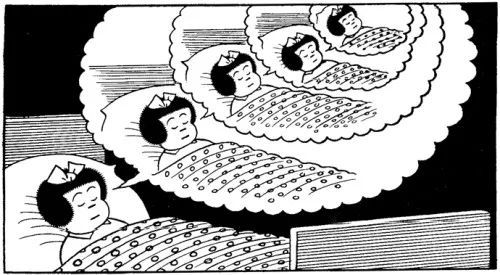
\includegraphics[scale=0.7]{img/Chapter5/5-3/1.png}
\end{figure}

\vspace{0.5cm}

\mybox{讲故事}

\begin{lstlisting}[language=Java]
public class TellStory {
	public static void main(String[] args) {
		tellStory();
	}

	public static void tellStory() {
		String story;
		story += "从前有座山,山里有座庙\n";
		story += "庙里有个老和尚\n";
		story += "老和尚在对小和尚讲故事:";
		System.out.println(story);

		tellStory();
	}
}
\end{lstlisting}

\begin{tcolorbox}
	\mybox{运行结果}
	\begin{verbatim}
从前有座山,山里有座庙
庙里有个老和尚
老和尚在对小和尚讲故事:
从前有座山,山里有座庙
庙里有个老和尚
老和尚在对小和尚讲故事:
从前有座山,山里有座庙
庙里有个老和尚
老和尚在对小和尚讲故事:
...
	\end{verbatim}
\end{tcolorbox}

一个永远无法结束的递归函数最终会导致栈溢出。因此递归函数需要确定一个结束条件,确保在递归过程中能在合适的地方停止并返回。\\

\mybox{阶乘}

\begin{lstlisting}[language=Java]
public class Factorial {
	public static void main(String[] args) {
		System.out.println("5! = " + factorial(5));
	}

	public static int factorial(int n) {
		if (n == 0 || n == 1) {
			return 1;
		}
		return n * factorial(n - 1);
	}
}
\end{lstlisting}

\begin{tcolorbox}
	\mybox{运行结果}
	\begin{verbatim}
5! = 120
	\end{verbatim}
\end{tcolorbox}

\begin{figure}[H]
	\centering
	\begin{tikzpicture}[]
		\draw (0,0) rectangle (3,1.5);
		\draw (3,-2) rectangle (6,-0.5);
		\draw (6,-4) rectangle (9,-2.5);
		\draw (9,-6) rectangle (12,-4.5);
		\draw (12,-8) rectangle (15,-6.5);

		\draw (12.75,-10.75) rectangle (14.25,-9.25);
		\draw (9.75,-8.75) rectangle (11.25,-7.25);
		\draw (6.75,-6.75) rectangle (8.25,-5.25);
		\draw (3.75,-4.75) rectangle (5.25,-3.25);
		\draw (0.75,-2.75) rectangle (2.25,-1.25);

		\draw (1.5,0.75) node {$ factorial(5) $};
		\draw (4.5,-1.25) node {$ factorial(4) $};
		\draw (7.5,-3.25) node {$ factorial(3) $};
		\draw (10.5,-5.25) node {$ factorial(2) $};
		\draw (13.5,-7.25) node {$ factorial(1) $};

		\draw (13.5,-10) node {$ 1 $};
		\draw (10.5,-8) node {$ 2 $};
		\draw (7.5,-6) node {$ 6 $};
		\draw (4.5,-4) node {$ 24 $};
		\draw (1.5,-2) node {$ 120 $};

		\draw[->] (3,0.75) -- (4.5,0.75) -- (4.5,-0.5);
		\draw[->] (6,-1.25) -- (7.5,-1.25) -- (7.5,-2.5);
		\draw[->] (9,-3.25) -- (10.5,-3.25) -- (10.5,-4.5);
		\draw[->] (12,-5.25) -- (13.5,-5.25) -- (13.5,-6.5);

		\draw[->] (12.75,-10) -- (10.5,-10) -- (10.5,-8.75);
		\draw[->] (9.75,-8) -- (7.5,-8) -- (7.5,-6.75);
		\draw[->] (6.75,-6) -- (4.5,-6) -- (4.5,-4.75);
		\draw[->] (3.75,-4) -- (1.5,-4) -- (1.5,-2.75);

		\draw (4.5,1) node {$ 5 * factorial(4) $};
		\draw (7.5,-1) node {$ 4 * factorial(3) $};
		\draw (10.5,-3) node {$ 3 * factorial(2) $};
		\draw (13.5,-5) node {$ 2 * factorial(1) $};

		\draw (11,-10.5) node {$ 2 * 1 $};
		\draw (8,-8.5) node {$ 3 * 2 $};
		\draw (5,-6.5) node {$ 4 * 6 $};
		\draw (2,-4.5) node {$ 5 * 24 $};
	\end{tikzpicture}
	\caption{阶乘}
\end{figure}

\vspace{0.5cm}

\mybox{斐波那契数列}

\begin{lstlisting}[language=Java]
public class Fibonacci {
	public static void main(String[] args) {
		int n = 7;
		System.out.println(fibonacci(n));
	}

	public static int fibonacci(int n) {
		if (n == 1 || n == 2) {
			return n;
		}
		return fibonacci(n - 2) + fibonacci(n - 1);
	}
}
\end{lstlisting}

\begin{tcolorbox}
	\mybox{运行结果}
	\begin{verbatim}
21
	\end{verbatim}
\end{tcolorbox}

\begin{figure}[H]
	\centering
	\begin{tikzpicture}[
			level distance=2.4cm,
			level 1/.style={sibling distance=6cm},
			level 2/.style={sibling distance=3cm},
			level 3/.style={sibling distance=2cm}
		]
		\node {$ f(5) $}
		child {
				node {$ f(3) $}
				child {node {$ f(1) $}}
				child {node {$ f(2) $}}
			}
		child {
				node {$ f(4) $}
				child {node {$ f(2) $}}
				child {
						node {$ f(3) $}
						child {node {$ f(1) $}}
						child {node {$ f(2) $}}
					}
			};
	\end{tikzpicture}
	\caption{递归树}
\end{figure}

递归的特点就是将一个复杂的大问题逐步简化为一个可以解决的小问题,然后再逐步计算出大问题的解。\\

递归的优点在于代码简洁易懂,但是缺点也很明显,就是效率很低。每次递归都会产生函数调用,而函数调用的开销是很大的,不适合用来解决大规模的问题。\\

例如在计算斐波那契数列的第40项时,递归需要花费大量时间,因为其中包含了大量的重复计算。相比而言,使用循环的方式能够节省大量的时间。因此像阶乘和斐波那契数列这样的情况,通常会采用循环,而不是递归进行计算。\\

然而还存在很多问题不得不使用递归的思想才能解决。\\

\mybox{阿克曼函数}

\begin{align}\nonumber
	A(m, n) =
	\begin{cases}
		n + 1             & m = 0        \\
		A(m-1, 1)         & m > 0, n = 0 \\
		A(m-1, A(m, n-1)) & m > 0, n > 0 \\
	\end{cases}
\end{align}

\begin{lstlisting}[language=Java]
public class Ackermann {
	public static void main(String[] args) {
		System.out.println(A(3, 4));
	}

	public static int A(int m, int n) {
		if (m == 0) {
			return n + 1;
		} else if (m > 0 && n == 0) {
			return A(m - 1, 1);
		} else {
			return A(m - 1, A(m, n - 1));
		}
	}
}
\end{lstlisting}

\begin{tcolorbox}
	\mybox{运行结果}
	\begin{verbatim}
125
	\end{verbatim}
\end{tcolorbox}

\vspace{0.5cm}

\mybox{汉诺塔}\\

有三根柱子A、B、C,A柱子上从下到上套有n个圆盘,要求将A柱子上的圆盘移动到C柱子上。每次只能移动一个圆盘,且大圆盘始终不能叠在小圆盘上面。\\

\begin{figure}[H]
	\centering
	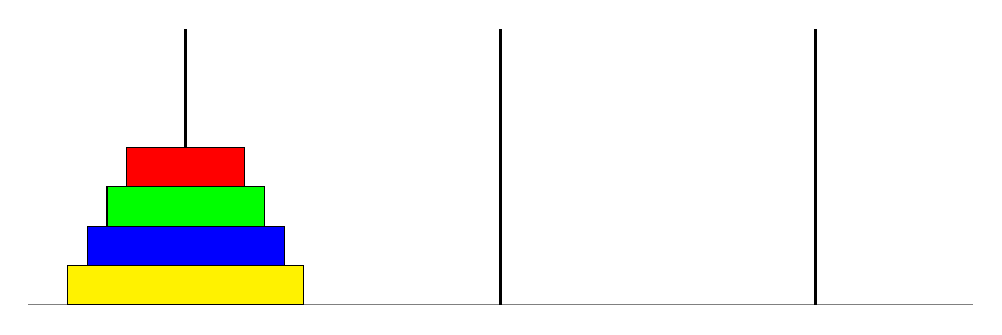
\begin{tikzpicture}[scale=0.5]
		\draw[-, gray] (0,0) -- (24,0);
		\draw[-, very thick] (4,0) -- (4,7);
		\draw[-, very thick] (12,0) -- (12,7);
		\draw[-, very thick] (20,0) -- (20,7);

		\draw[fill=red] (2.5,3) rectangle (5.5,4);
		\draw[fill=green] (2,2) rectangle (6,3);
		\draw[fill=blue] (1.5,1) rectangle (6.5,2);
		\draw[fill=yellow] (1,0) rectangle (7,1);
	\end{tikzpicture}
	\caption{汉诺塔}
\end{figure}

递归算法求解汉诺塔问题:

\begin{enumerate}
	\item 将n-1个圆盘从A借助C移到B。
	\item 将第n个圆盘从A移到C。
	\item 将n-1个圆盘从B借助A移到C。
\end{enumerate}

\vspace{-0.5cm}

\begin{lstlisting}[language=Java]
public class Hanoi {
	static int move = 0;

	public static void main(String[] args) {
		hanoi(3, 'A', 'B', 'C');
		System.out.println("Moves: " + move);
	}

	public static void hanoi(int n, char src, char mid, char dst) {
		if (n == 1) {
			System.out.println(src + " -> " + dst);
			move++;
		} else {
			// move top n-1 disks from src to mid
			hanoi(n - 1, src, dst, mid);
			System.out.println(src + " -> " + dst);
			move++;
			// move top n-1 disks from mid to dst
			hanoi(n - 1, mid, src, dst);
		}
	}
}
\end{lstlisting}

\begin{tcolorbox}
	\mybox{运行结果}
	\begin{verbatim}
A -> C
A -> B
C -> B
A -> C
B -> A
B -> C
A -> C
Moves: 7
	\end{verbatim}
\end{tcolorbox}

假设每次移动花费1秒,解决一个64层的汉诺塔问题大约需要5800亿年。\\

\begin{figure}[H]
	\centering
	
\includegraphics[]{img/Chapter5/5-3/2.png}
\end{figure}

\newpage
\chapter{面向对象}

\section{封装}

\subsection{类与对象}

在面向对象编程中,把构成问题的事物分解成各个对象,每个对象都有自己的数据和行为,程序通过对象之间的交互来实现功能。\\

类(class)是一个模板,定义了对象的属性和方法,用来描述同一类对象的共同特征和行为。对象(object)是类的实例,它具有类定义的属性和方法。\\

关键字new可以实例化一个类对象,之后就可以通过访问对象的属性和方法来操作对象。\\

\mybox{银行账户}

\begin{lstlisting}[language=Java]
public class BankAccount {
    String owner;
    String account;
    double balance;

    public void deposit(double amount) {
        balance += amount;
    }

    public void withdraw(double amount) {
        balance -= amount;
    }
}
\end{lstlisting}

\begin{lstlisting}[language=Java]
public class Bank {
    public static void main(String[] args) {
        BankAccount account = new BankAccount();
        account.owner = "Terry";
        account.account = "6250941006528599";
        account.balance = 50;

        System.out.println("Owner: " + account.owner);
        System.out.println("Account: " + account.account);
        System.out.println("Balance: " + account.balance);

        account.deposit(100);
        System.out.println("Balance: " + account.balance);

        account.withdraw(70);
        System.out.println("Balance: " + account.balance);
    }
}
\end{lstlisting}

\begin{tcolorbox}
    \mybox{运行结果}
    \begin{verbatim}
Owner: Terry
Account: 6250941006528599
Balance: 50.0
Balance: 150.0
Balance: 80.0
\end{verbatim}
\end{tcolorbox}

\vspace{0.5cm}

\subsection{封装(Encapsulation)}

封装是面向对象的重要原则,尽可能隐藏对象的内部实现细节。封装可以认为是一个保护屏障,防止该类的数据被外部随意访问。当要访问该类的数据时,必须通过指定的接口。合适的封装可以让代码更容易理解和维护,也加强了程序的安全性。\\

为了实现封装,需要对类的属性和方法进行访问权限的控制:

\begin{enumerate}
    \item public:允许任何地方访问。
    \item private:只允许在类的内部访问。
    \item protected:只允许在类的内部和子类中访问。
    \item default:只允许在同一个包中访问。
\end{enumerate}

通常会将类的属性设置为private,然后对外提供一对setter/getter方法来访问该属性。\\

为了避免方法的参数与类的属性重名造成歧义,可以使用this关键字用来指代当前对象。\\

\mybox{银行账户}

\begin{lstlisting}[language=Java]
public class BankAccount {
    private final int ACCOUNT_DIGITS = 16;

    private String owner;
    private String account;
    private double balance;

    public void setOwner(String owner) {
        if (!owner.isEmpty()) {
            this.owner = owner;
        }
    }

    public String getOwner() {
        return owner;
    }

    public void setaccount(String account) {
        if (account.length() == ACCOUNT_DIGITS) {
            this.account = account;
        }
    }

    public String getAccount() {
        return account;
    }

    public void setBalance(double balance) {
        if (balance >= 0) {
            this.balance = balance;
        }
    }

    public double getBalance() {
        return balance;
    }

    public boolean deposit(double amount) {
        if (amount <= 0) {
            return false;
        }
        balance += amount;
        return true;
    }

    public boolean withdraw(double amount) {
        if (amount <= 0 || amount > balance) {
            return false;
        }
        balance -= amount;
        return true;
    }
}
\end{lstlisting}

\begin{lstlisting}[language=Java]
public class Bank {
    public static void main(String[] args) {
        BankAccount account = new BankAccount();
        account.setOwner("Terry");
        account.setAccount("6250941006528599");
        account.setBalance(50);

        System.out.println("Owner: " + account.getOwner());
        System.out.println("Account: " + account.getAccount());
        System.out.println("Balance: " + account.getBalance());

        account.deposit(100);
        System.out.println("Balance: " + account.getBalance());

        account.withdraw(70);
        System.out.println("Balance: " + account.getBalance());
    }
}
\end{lstlisting}

\begin{tcolorbox}
    \mybox{运行结果}
    \begin{verbatim}
Owner: Terry
Account: 6250941006528599
Balance: 50.0
Balance: 150.0
Balance: 80.0
\end{verbatim}
\end{tcolorbox}

\newpage

\section{构造方法}

\subsection{构造方法(Constructor)}

构造方法是一种特殊的方法,会在创建对象时自动调用,用于创建并初始化对象。每个类可以有一个或多个构造方法,构造方法的名字必须和类名一致。构造方法没有返回值,返回值类型部分不写。

\vspace{-0.5cm}

\begin{lstlisting}[language=Java]
public BankAccount() {
    owner = "admin";
    account = "0000000000000000";
    balance = 0;
}
\end{lstlisting}

如果一个类中没有写构造方法,系统会自动提供一个public的无参构造方法,以便实例化对象。如果一个类中已经写了构造方法,系统将不会再提供默认的无参构造方法。

\vspace{-0.5cm}

\begin{lstlisting}[language=Java]
public BankAccount(String owner, String account, double balance) {
    if (!owner.isEmpty()) {
        this.owner = owner;
    }

    if (account.length() == ACCOUNT_DIGITS) {
        this.account = account;
    }

    if (balance >= 0) {
        this.balance = balance;
    }
}
\end{lstlisting}

\vspace{0.5cm}

\subsection{重载(Overload)}

重载用于在同一个类定义多个同名方法,但是这些方法的参数列表不同。重载的主要用途是提供方法的多种版本,以便满足不同的需求。\\

重载还可以使代码更具可读性,因为它使得方法名更具描述性,而不必考虑特定的参数列表。\\

\mybox{银行账户}

\begin{lstlisting}[language=Java]
public class BankAccount {
    private final int ACCOUNT_DIGITS = 16;

    private String owner;
    private String account;
    private double balance;

    public BankAccount() {
        owner = "admin";
        account = "0000000000000000";
        balance = 0;
    }

    public BankAccount(String owner, String account, double balance) {
        if (!owner.isEmpty()) {
            this.owner = owner;
        }

        if (account.length() == ACCOUNT_DIGITS) {
            this.account = account;
        }

        if (balance >= 0) {
            this.balance = balance;
        }
    }

    public void setOwner(String owner) {
        if (!owner.isEmpty()) {
            this.owner = owner;
        }
    }

    public String getOwner() {
        return owner;
    }

    public void setAccount(String account) {
        if (account.length() == ACCOUNT_DIGITS) {
            this.account = account;
        }
    }

    public String getAccount() {
        return account;
    }

    public void setBalance(double balance) {
        if (balance >= 0) {
            this.balance = balance;
        }
    }

    public double getBalance() {
        return balance;
    }

    public boolean deposit(double amount) {
        if (amount <= 0) {
            return false;
        }
        balance += amount;
        return true;
    }

    public boolean withdraw(double amount) {
        if (amount <= 0 || amount > balance) {
            return false;
        }
        balance -= amount;
        return true;
    }

    public boolean withdraw(double amount, double fee) {
        if(amount <= 0 || amount + fee > balance) {
            return false;
        }

        balance -= amount + fee;
        return true;
    }
}
\end{lstlisting}

\begin{lstlisting}[language=Java]
public class Bank {
    public static void main(String[] args) {
        BankAccount account1 = new BankAccount();
        System.out.println(
                "Account 1 Owner: " + account1.getOwner()
        );
        System.out.println(
                "Account 1 Account: " + account1.getAccount()
        );
        System.out.println(
                "Account 1 Balance: " + account1.getBalance()
        );

        BankAccount account2 = new BankAccount(
                "Terry", "6250941006528599", 50
        );
        System.out.println(
                "Account 2 Balance: " + account2.getBalance()
        );

        account2.withdraw(20);
        System.out.println(
                "Account 2 Balance: " + account2.getBalance()
        );

        account2.withdraw(10, 1);
        System.out.println(
                "Account 2 Balance: " + account2.getBalance()
        );
    }
}
\end{lstlisting}

\begin{tcolorbox}
    \mybox{运行结果}
    \begin{verbatim}
Account 1 Owner: admin
Account 1 Account: 0000000000000000
Account 1 Balance: 0.0
Account 2 Balance: 50.0
Account 2 Balance: 30.0
Account 2 Balance: 19.0  
	\end{verbatim}
\end{tcolorbox}

\newpage

\section{继承}

\subsection{继承(Inheritance)}

继承指一个类可以继承另一个类的特征和行为,并可以对其进行扩展。这样就可以避免在多个类中重复定义相同的特征和行为。\\

\begin{figure}[H]
    \centering
    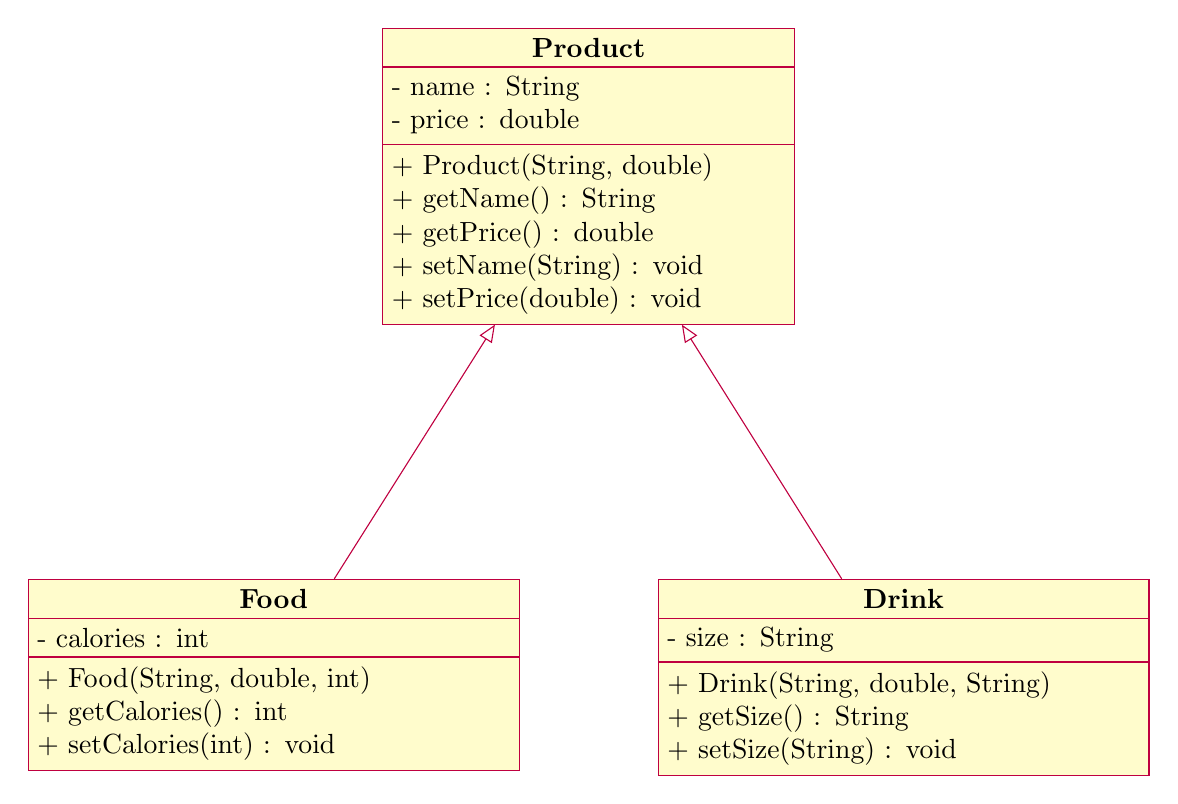
\begin{tikzpicture}
        \begin{class}[text width = 5cm]{Product}{0,0}
            \attribute{- name : String}
            \attribute{- price : double}
            \operation{+ Product(String, double)}
            \operation{+ getName() : String}
            \operation{+ getPrice() : double}
            \operation{+ setName(String) : void}
            \operation{+ setPrice(double) : void}
        \end{class}

        \begin{class}[text width = 6cm]{Food}{-4,-7}
            \inherit{Product}
            \attribute{- calories : int}
            \operation{+ Food(String, double, int)}
            \operation{+ getCalories() : int}
            \operation{+ setCalories(int) : void}
        \end{class}

        \begin{class}[text width = 6cm]{Drink}{4,-7}
            \inherit{Product}
            \attribute{- size : String}
            \operation{+ Drink(String, double, String)}
            \operation{+ getSize() : String}
            \operation{+ setSize(String) : void}
        \end{class}
    \end{tikzpicture}
    \caption{继承}
\end{figure}

extends关键字用于指定一个类继承于另一个类,产生继承关系后,子类可以通过super关键字调用父类中的属性和方法,也可以定义子类独有的属性和方法。\\

在创建子类对象时,会先调用父类的构造方法,然后再调用子类的构造方法。因此父类中必须存在一个构造方法,否则将无法创建子类对象。\\

\mybox{麦当劳}

\begin{lstlisting}[language=Java]
public class Product {
    private String name;
    private double price;

    public Product(String name, double price) {
        this.name = name;
        this.price = price;
    }

    public String getName() {
        return name;
    }

    public void setName(String name) {
        this.name = name;
    }

    public double getPrice() {
        return price;
    }

    public void setPrice(double price) {
        this.price = price;
    }
}
\end{lstlisting}

\begin{lstlisting}[language=Java]
public class Food extends Product {
    int calories;

    public Food(String name, double price, int calories) {
        super(name, price);
        this.calories = calories;
    }

    public int getCalories() {
        return calories;
    }

    public void setCalories(int calories) {
        this.calories = calories;
    }
}
\end{lstlisting}

\begin{lstlisting}[language=Java]
public class Drink extends Product {
    private String size;

    public Drink(String name, double price, String size) {
        super(name, price);
        this.size = size;
    }

    public String getSize() {
        return size;
    }

    public void setSize(String size) {
        this.size = size;
    }
}
\end{lstlisting}

\begin{lstlisting}[language=Java]
public class McDonalds {
    public static void main(String[] args) {
        Food food = new Food("Cheeseburger", 5.45, 302);
        Drink drink = new Drink("Coke", 3.7, "Large");

        System.out.printf(
                "Food: %s ($%.2f) %d Kcal\n",
                food.getName(), food.getPrice(), food.getCalories()
        );
        System.out.printf(
                "Drink: %s ($%.2f) %s\n",
                drink.getName(), drink.getPrice(), drink.getSize()
        );
    }
}
\end{lstlisting}

\begin{tcolorbox}
    \mybox{运行结果}
    \begin{verbatim}
Food: Cheeseburger ($5.45) 302 Kcal
Drink: Coke ($3.70) Large
	\end{verbatim}
\end{tcolorbox}

\vspace{0.5cm}

\subsection{重写(Override)}

Object类是所有类的根类,所有的类都直接或者间接地继承自Object类。Object类中包含的方法在其它所有类中都可以使用,例如getClass()、hashCode()、toString()、clone()、equals()等。\\

当直接输出一个对象时,会自动调用该对象的toString()方法,将其以字符串的形式输出。

\vspace{-0.5cm}

\begin{lstlisting}[language=Java]
System.out.println(food);   // Food@41629346
\end{lstlisting}

在没有重写toString()方法的情况下,输出的内容是对象的类名及其哈希码(hash code),但这并不是预期想要的结果。因此,可以重写从父类继承的toString(),以满足程序的需求。\\

在重写方法时,需要使用@Override注解,以便编译器检查该方法是否真的是从父类继承的。\\

Object类的equals()方法默认比较的是两个对象的地址,如果地址相同则为true,否则为false。而String类的equals()方法就重写了Object类的equals()方法,以便比较两个字符串的内容是否相同。\\

\mybox{麦当劳}

\begin{lstlisting}[language=Java]
public class Product {
    private String name;
    private double price;

    public Product(String name, double price) {
        this.name = name;
        this.price = price;
    }

    public String getName() {
        return name;
    }

    public void setName(String name) {
        this.name = name;
    }

    public double getPrice() {
        return price;
    }

    public void setPrice(double price) {
        this.price = price;
    }

    @Override
    public String toString() {
        return String.format("%s ($%.2f)", name, price);
    }
}
\end{lstlisting}

\begin{lstlisting}[language=Java]
public class Food extends Product {
    int calories;

    public Food(String name, double price, int calories) {
        super(name, price);
        this.calories = calories;
    }

    public int getCalories() {
        return calories;
    }

    public void setCalories(int calories) {
        this.calories = calories;
    }

    @Override
    public String toString() {
        return "Food: " + super.toString() + " " + calories + " Kcal";
    }
}
\end{lstlisting}

\begin{lstlisting}[language=Java]
public class Drink extends Product {
    private String size;

    public Drink(String name, double price, String size) {
        super(name, price);
        this.size = size;
    }

    public String getSize() {
        return size;
    }

    public void setSize(String size) {
        this.size = size;
    }

    @Override
    public String toString() {
        return "Drink: " + super.toString() + " " + size;
    }
}
\end{lstlisting}

\begin{lstlisting}[language=Java]
public class McDonalds {
    public static void main(String[] args) {
        Food food = new Food("Cheeseburger", 5.45, 302);
        Drink drink = new Drink("Coke", 3.7, "Large");

        System.out.println(food);
        System.out.println(drink);
    }
}
\end{lstlisting}

\begin{tcolorbox}
    \mybox{运行结果}
    \begin{verbatim}
Food: Cheeseburger ($5.45) 302 Kcal
Drink: Coke ($3.70) Large
	\end{verbatim}
\end{tcolorbox}

\newpage

\section{抽象类}

\subsection{抽象类(Abstract Class)}

有些类只能用来做继承,不能用于创建对象。例如在动物园中并不存在“动物”这个对象,只有动物的子类对象,因此动物类不应该被实例化。\\

抽象类是一种不能被实例化的类,它用于定义接口或公共实现,供其它类继承并实现。

\vspace{-0.5cm}

\begin{lstlisting}[language=Java]
public abstract class Animal {}
\end{lstlisting}

\vspace{0.5cm}

\subsection{抽象方法}

有时候父类提供的方法无法满足子类不同的需求,但是如果不定义该方法,就表示该类具有该行为。\\

这种情况就可以将这个父类的方法定义为抽象方法,这样所有的子类都必须要重写该方法,否则子类仍然为抽象类。\\

抽象方法只需声明,而不用实现。包含抽象方法的类必须声明为抽象类。\\

\mybox{动物}

\begin{lstlisting}[language=Java]
public abstract class Animal {
    public abstract String sound();
}
\end{lstlisting}

\begin{lstlisting}[language=Java]
public class Dog extends Animal {
    @Override
    public String sound() {
        return "Woof";
    }
}
\end{lstlisting}

\begin{lstlisting}[language=Java]
public class Cat extends Animal {
    @Override
    public String sound() {
        return "Meow";
    }
}
\end{lstlisting}

\begin{lstlisting}[language=Java]
public class AnimalSound {
    public static void main(String[] args) {
        Dog dog = new Dog();
        Cat cat = new Cat();

        System.out.println("Dog's sound: " + dog.sound());
        System.out.println("Cat's sound: " + cat.sound());
    }
}
\end{lstlisting}

\begin{tcolorbox}
    \mybox{运行结果}
    \begin{verbatim}
Dog's sound: Woof
Cat's sound: Meow
	\end{verbatim}
\end{tcolorbox}

\newpage

\section{多态}

\subsection{多态(Polymorphism)}

多态是指对象可以具有多种形态,即同一个对象在不同时刻表现出不同的行为。例如Dog和Cat都是Animal的子类,因此可以将子类对象赋值给父类引用,从而产生多种形态。

\vspace{-0.5cm}

\begin{lstlisting}[language=Java]
Animal animal = new Dog();
\end{lstlisting}

由子类类型转型为父类类型,称为向上转型。向上转型是一种隐式转换,向上转型后的对象,只能访问父类中定义的成员。\\

由父类类型转型为子类类型,称为向下转型。向下转型存在失败的可能,因为父类对象并不一定是子类对象。\\

向下转型需要显式地强制转换,在转换时需要使用instanceof关键字进行类型检查。\\

\mybox{员工工资}

\begin{lstlisting}[language=Java]
public abstract class Employee {
    private String name;

    public Employee(String name) {
        this.name = name;
    }

    public String getName() {
        return name;
    }

    public abstract double getSalary();
}
\end{lstlisting}

\begin{lstlisting}[language=Java]
public class FullTimeEmployee extends Employee {
    private double basicSalary;
    private double bonus;

    public FullTimeEmployee(
            String name, double basicSalary, double bonus
    ) {
        super(name);
        this.basicSalary = basicSalary;
        this.bonus = bonus;
    }

    @Override
    public double getSalary() {
        return basicSalary + bonus;
    }
}
\end{lstlisting}

\begin{lstlisting}[language=Java]
public class PartTimeEmployee extends Employee {
    private double dailyWage;
    private int workingDays;

    public PartTimeEmployee(
            String name, double dailyWage, int workingDays
    ) {
        super(name);
        this.dailyWage = dailyWage;
        this.workingDays = workingDays;
    }

    @Override
    public double getSalary() {
        return dailyWage * workingDays;
    }
}
\end{lstlisting}

\begin{lstlisting}[language=Java]
public class Salary {
    public static void main(String[] args) {
        Employee[] employees = new Employee[]{
                new FullTimeEmployee("Alice", 5783, 173),
                new PartTimeEmployee("Bob", 150, 15)
        };

        for (Employee employee : employees) {
            System.out.println(
                    employee.getName() + ": $" + employee.getSalary()
            );
        }
    }
}
\end{lstlisting}

\begin{tcolorbox}
    \mybox{运行结果}
    \begin{verbatim}
Alice: $5956.0
Bob: $2250.0
	\end{verbatim}
\end{tcolorbox}

\newpage

\section{接口}

\subsection{接口(Interface)}

接口是一种特殊的抽象类,接口中的所有方法都是抽象方法,接口中的成员变量必须是常量。\\

接口用于定义一组标准,代表了某种能力和约定。例如USB接口代表了电脑和外设设备之间的连接标准。USB接口不用关心连接的外设设备是什么,只要这个外设设备满足USB的标准,就可以连接到电脑上。\\

\mybox{USB}

\begin{lstlisting}[language=Java]
public interface USB {
    String getDeviceInfo();
}
\end{lstlisting}

\begin{lstlisting}[language=Java]
public class Mouse implements USB {
    @Override
    public String getDeviceInfo() {
        return "Mouse";
    }
}
\end{lstlisting}

\begin{lstlisting}[language=Java]
public class Keyboard implements USB {
    @Override
    public String getDeviceInfo() {
        return "Keyboard";
    }
}
\end{lstlisting}

\begin{lstlisting}[language=Java]
public class Computer {
    private USB usb1;
    private USB usb2;

    public void setUSB1(USB usb) {
        usb1 = usb;
    }

    public void setUSB2(USB usb) {
        usb2 = usb;
    }

    @Override
    public String toString() {
        return "USB 1: " + usb1.getDeviceInfo() + "\n"
                + "USB 2: " + usb2.getDeviceInfo();
    }

    public static void main(String[] args) {
        Computer computer = new Computer();

        computer.setUSB1(new Mouse());
        computer.setUSB2(new Keyboard());

        System.out.println(computer);
    }
}
\end{lstlisting}

\begin{tcolorbox}
    \mybox{运行结果}
    \begin{verbatim}
USB 1: Mouse
USB 2: Keyboard
	\end{verbatim}
\end{tcolorbox}

\newpage
\chapter{封装}

\section{面向过程与面向对象}

\subsection{面向过程(Procedure Oriented)}

面向过程是一种以过程为中心的编程思想,以什么正在发生为主要目标进行编程,分析出解决问题所需要的步骤,然后用函数把这些步骤一步一步实现,使用的时候一个一个依次调用。 \\

C语言就是一种面向过程的编程语言,但是面向过程的缺陷是数据和函数并不完全独立,使用两个不同的实体表示信息及其操作。

\subsection{面向对象(Object Oriented)}

面向对象是相对于面向过程来讲的,面向对象方法把相关的数据和方法组织为一个整体来看待,从更高的层次来进行系统建模,更贴近事物的自然运行模式。 \\

在面向对象中,把构成问题的事物分解成各个对象,建立对象的目的不是为了完成一个步骤,而是为了描叙某个事物在整个解决问题的步骤中的行为。 \\

Java、C++、Python等都是面向对象的编程语言,面向对象的优势在于只是用一个实体就能同时表示信息及其操作。 \\

面向对象三大特性:

\begin{enumerate}
    \item 封装(encapsulation):数据和代码捆绑,避免外界干扰和不确定性访问。
    \item 继承(inheritance):让某种类型对象获得另一类型对象的属性和方法。
    \item 多态(polymorphism):同一事物表现出不同事物的能力。
\end{enumerate}

\newpage

\section{类与对象}

\subsection{类与对象}

类(class)表示同一类具有相同特征和行为的对象的集合,类定义了对象的属性和方法。 \\

对象(object)是类的实例,对象拥有属性和方法。 \\

类的设计需要使用关键字class,类名是一个标识符,遵循大驼峰命名法。类中可以包含属性和方法。其中,属性通过变量表示,又称实例变量;方法用于描述行为,又称实例方法。 \\

通过关键字new进行对象的实例化,实例化对象会调用类中的构造函数完成。类是一种引用数据类型,对象的实例化在堆上开辟空间。 \\

\mybox{类和对象}

\begin{lstlisting}[language=Java, title=Person.java]
public class Person {
    // 属性:描述所有对象共有的特征
    public String name;
    public int age;
    public String gender;

    // 方法:描述所有对象共有的功能
    public void eat() {
        System.out.println("吃饭");
    }

    public void sleep() {
        System.out.println("睡觉");
    }
}
\end{lstlisting}

\begin{lstlisting}[language=Java, title=TestPerson.java]
public class TestPerson {
    public static void main(String[] args) {
        Person zhangsan = new Person();
        zhangsan.name = "张三";
        zhangsan.age = 18;
        zhangsan.gender = "男";

        Person lisi = new Person();
        lisi.name = "李四";
        lisi.age = 22;
        lisi.gender = "女";

        System.out.println("姓名:" + zhangsan.name 
                            + " 年龄:" + zhangsan.age
                            + " 性别:" + zhangsan.gender);
        System.out.println("姓名:" + lisi.name 
                            + " 年龄:" + lisi.age
                            + " 性别:" + lisi.gender);
        
        zhangsan.eat();
        lisi.sleep();
    }
}
\end{lstlisting}

\begin{tcolorbox}
	\mybox{运行结果}
	\begin{verbatim}
姓名:张三 年龄:18 性别:男
姓名:李四 年龄:22 性别:女
吃饭
睡觉
	\end{verbatim}
\end{tcolorbox}

\newpage

\section{封装}

\subsection{封装(Encapsulation)}

封装是面向对象方法的重要原则,就是把对象的属性和方法结合为一个独立的整体,并尽可能隐藏对象的内部实现细节。 \\

封装可以认为是一个保护屏障,防止该类的数据被外部类随意访问。要访问该类的数据,必须通过严格的接口控制。合适的封装可以让代码更容易理解和维护,也加强了程序的安全性。 \\

实现封装的步骤:

\begin{enumerate}
    \item 修改属性的可见性来限制对属性的访问,一般限制为private。
    \item 对每个属性提供对外的公共方法访问,也就是提供一对setter / getter,用于对私有属性的访问。
\end{enumerate}

\subsection{访问权限}

属性和方法的访问权限一般分为3种:

\begin{enumerate}
    \item public:属性和方法在类的内部和外部都可以访问。
    \item private:属性和方法只能在类内访问。
    \item protected:属性和方法只能在类的内部和其派生类中访问。
\end{enumerate}

\subsection{this指针}

每一个对象都能通过this指针来访问自身的地址,this指针是所有成员方法的隐含参数,在成员方法内部可以用来指向调用对象。 \\

在类中,属性的名字可以和局部变量的名字相同。此时,如果直接使用名字来访问,优先访问的是局部变量。因此,需要使用this指针来访问当前对象的属性。 \\

当需要访问的属性与局部变量没有重名的时候,this可以省略。 \\

\mybox{封装}

\begin{lstlisting}[language=Java, title=Person.java]
public class Person {
    private String name;
    private int age;

    public void setName(String name) {
        this.name = name;
    }

    public void setAge(int age) {
        this.age = age;
    }

    public String getName() {
        return name;
    }

    public int getAge() {
        return age;
    }
}
\end{lstlisting}

\begin{lstlisting}[language=Java, title=TestPerson.java]
public class TestPerson {
    public static void main(String[] args) {
        Person person = new Person();
        person.setName("小灰");
        person.setAge(17);
        System.out.println("姓名:" + person.getName());
        System.out.println("年龄:" + person.getAge());
    }
}
\end{lstlisting}

\begin{tcolorbox}
	\mybox{运行结果}
	\begin{verbatim}
姓名:小灰
年龄:17
	\end{verbatim}
\end{tcolorbox}

\newpage

\section{构造方法}

\subsection{构造方法(Constructor)}

构造方法也是一个方法,用于实例化对象,在实例化对象的时候调用。一般情况下,使用构造方法是为了在实例化对象的同时,给一些属性进行初始化赋值。 \\

构造方法和普通方法的区别:

\begin{enumerate}
    \item 构造方法的名字必须和类名一致。
    \item  构造方法没有返回值,返回值类型部分不写。
\end{enumerate}

如果一个类中没有写构造方法,系统会自动提供一个public权限的无参构造方法,以便实例化对象。如果一个类中已经写了构造方法,此时系统将不再提供任何默认的构造方法。 \\

\mybox{构造方法}

\begin{lstlisting}[language=Java, title=Person.java]
public class Person {
    private String name;
    private int age;
    
    /**
     * 无参构造方法
     */
    public Person() {
        this.name = "";
        this.age = 0;
    }

    /**
     * 有参构造方法
     */
    public Person(String name, int age) {
        this.name = name;
        this.age = age;
    }

    public void setName(String name) {
        this.name = name;
    }

    public void setAge(int age) {
        this.age = age;
    }

    public String getName() {
        return name;
    }

    public int getAge() {
        return age;
    }
}
\end{lstlisting}

\begin{lstlisting}[language=Java, title=TestPerson.java]
public class TestPerson {
    public static void main(String[] args) {
        Person person = new Person("小灰", 17);
        System.out.println("姓名:" + person.getName());
        System.out.println("年龄:" + person.getAge());
    }
}
\end{lstlisting}

\begin{tcolorbox}
	\mybox{运行结果}
	\begin{verbatim}
姓名:小灰
年龄:17
	\end{verbatim}
\end{tcolorbox}

\newpage
\chapter{多态}

\section{抽象类}

\subsection{多态(Polymorphism)}

多态是同一个行为具有多个不同表现形式或形态的能力。例如可以把一只哈士奇,当成它的父类去看待,因此哈士奇是一只狗、一个动物或一个生物。\\

通过父类引用指向子类对象,例如Animal animal = new Dog(),从而产生多种形态。父类引用仅能访问父类所声明的属性和方法,不能访问子类独有的属性和方法。\\

在一对有继承关系的类中都有一个方法,其方法名、参数列表、返回值均相同,通过调用方法实现不同类对象完成不同的事件。\\

\subsection{抽象类(Abstract Class)}

抽象类不能被用于实例化对象,只是提供了所有的子类共有的部分。例如在动物园中,存在的都是“动物”具体的子类对象,并不存在“动物”对象,所以动物类不应该被独立创建成对象。\\

抽象类的作用是可以被子类继承,提供共性的属性和方法。\\

\subsection{抽象方法(Abstract Method)}

父类提供的方法很难满足子类不同的需求,如果不定义该方法,则表示所有的子类都不具有该行为。如果定义该方法,所有的子类都在重写,那么这个方法在父类中是没有必要实现的,显得多余。\\

被abstract关键字修饰的方法称为抽象方法。抽象方法只有声明,没有实现。抽象方法只能包含在抽象类中。产生继承关系后,子类必须重写父类中所有的抽象方法,否则子类还是抽象类。\\

非抽象类在继承自一个抽象父类的同时,必须重写实现父类中所有的抽象方法。因此,抽象类可以用来做一些简单的规则制定。在抽象类中制定一些规则,要求所有的子类必须实现,约束所有子类的行为。\\

但是,类是单继承的,一个类有且只能有一个父类,所以如果一个类需要受到多种规则的约束,无法再继承其它父类。此时可以使用接口进行这样的复杂的规则制定。

\newpage

\section{对象转型}

\subsection{对象转型}

对象由子类类型转型为父类类型,即是向上转型。向上转型是一种隐式转换,一定会转型成功。向上转型后的对象,只能访问父类中定义的成员。\\

由父类类型转型转型为子类类型,即是向下转型。向下转型存在失败的可能性,会出现ClassCastException异常。向下转型需要进行强制类型转换,是一个显式转换。向下转型后的对象,将可以访问子类中独有的成员。\\

向下转型存在失败的可能性。如果引用实际指向的对象,不是要转型的类型,此时强制转换会出现ClassCastException异常。所以,在向下转型之前,最好使用instanceof关键字进行类型检查。\\

\mybox{对象转型}

\begin{lstlisting}[language=Java, title=Animal.java]
public abstract class Animal {
    private String name;

    public Animal(String name) {
        this.name = name;
    }

    public abstract void makeSound();
}
\end{lstlisting}

\begin{lstlisting}[language=Java, title=Dog.java]
public class Dog extends Animal {
    public Dog(String name) {
        super(name);
    }
    
    @Override
    public void makeSound() {
        System.out.println("汪汪~");
    }
}
\end{lstlisting}

\begin{lstlisting}[language=Java, title=TestDog.java]
public class TestDog {
    public static void main(String[] args) {
        Animal animal = new Dog("狗子");
        if(animal instanceof Dog) {
            Dog dog = (Dog)animal;
            dog.makeSound();
        }
    }
}
\end{lstlisting}

\begin{tcolorbox}
	\mybox{运行结果}
	\begin{verbatim}
汪汪~
	\end{verbatim}
\end{tcolorbox}

\newpage

\section{接口}

\subsection{接口}

在面向对象中会使用抽象类为外部提供一个通用的、标准化的接口。\\

宏观上来讲,接口是一种标准。例如常见的USB接口,电脑通过USB接口连接各种外设设备,每一个接口不用关心连接的外设设备是什么,只要这个外设设备实现了USB的标准,就可以连接到电脑上。\\

从程序上来讲,接口代表了某种能力和约定。当父类的方法无法满足子类需求时,可实现接口扩充子类的能力,接口中方法的定义代表能力的具体要求。\\

定义接口需要使用关键字interface,接口中可以定义:

\begin{enumerate}
	\item 属性:默认都是静态常量,访问权限都是public。
	\item 方法:默认都是抽象方法,访问权限都是public。
\end{enumerate}

接口和抽象类的相同点有:

\begin{enumerate}
	\item 都不能创建对象。
	\item 都具备Object类中所定义的方法。
	\item 都可以写抽象方法。
\end{enumerate}

接口和抽象类的不同点有:

\begin{enumerate}
	\item 接口中所有的属性都是公开静态常量,缺省用public static final修饰。
	\item 接口中所有的方法都是公开抽象方法,缺省用public abstract修饰。
	\item 接口中没有构造方法、构造代码段和静态代码段。
\end{enumerate}

因为接口中有很多抽象方法,因此非抽象类在实现接口的时候必须重写实现接口中所有的抽象方法。\\

使用接口可以进行对行为的约束和规则的制定,接口表示一组能力,那么一个类可以接受多种能力的约束。因此一个类可以实现多个接口,实现多个接口的时候,必须要把每一个接口中的方法都实现。如果一个类实现的多个接口中有相同的方法,实现类只需实现一次即可。\\

\mybox{接口}

\begin{lstlisting}[language=Java, title=USB.java]
public interface USB {
    /**
     * USB接口返回当前连接设备的类型
     * @return 当前连接设备
     */
    String getDeviceInfo();
}
\end{lstlisting}

\begin{lstlisting}[language=Java, title=Mouse.java]
public class Mouse implements USB {
    @Override
    public String getDeviceInfo() {
        return "mouse";
    }
}
\end{lstlisting}

\begin{lstlisting}[language=Java, title=Keyboard.java]
public class Keyboard implements USB {
    @Override
    public String getDeviceInfo() {
        return "keyboard";
    }
}
\end{lstlisting}

\begin{lstlisting}[language=Java, title=Computer.java]
public class Computer {
    // 电脑有2个USB接口
    private USB usb1;
    private USB usb2;
    
    public void setUsb1(USB usb1) {
        this.usb1 = usb1;
    }
    
    public void setUsb2(USB usb2) {
        this.usb2 = usb2;
    }
    
    /**
     * 获取USB接口连接设备的信息
     */
    public String getUsbInfo() {
        return "USB 1: " + this.usb1.getDeviceInfo() + "\n"
                + "USB 2: " + this.usb2.getDeviceInfo();
    }
}
\end{lstlisting}

\begin{lstlisting}[language=Java, title=TestUsb.java]
public class TestUsb {
    public static void main(String[] args) {
        Computer computer = new Computer();
        
        // 外设设备连接到电脑上
        computer.setUsb1(new Mouse());
        computer.setUsb2(new Keyboard());
        
        System.out.println(computer.getUsbInfo());
    }
}
\end{lstlisting}

\begin{tcolorbox}
	\mybox{运行结果}
	\begin{verbatim}
USB 1: mouse
USB 2: keyboard
	\end{verbatim}
\end{tcolorbox}

\newpage

\end{document}